%
% Perspective
%

% !TEX root = ../../main.tex

\chapter{Diskussion und Ausblick\label{chap:perspective}}

  \section{Diskussion der Resultate\label{sec:diskRes}}

    Die gefundenen Resultate wiederspiegeln Lösungen innerhalb einer künstlichen Umgebung.
    In dieser Umgebung wird eine vereinfachte Physik verwendet, welche nur eine Annäherung an die reale Physik ist.
    Deshalb sind die Resultate nicht ohne Vorbehalte auf die reale Welt übertragbar.
    \\
    Das Evolvieren von artifiziellen Tieren und ihrer Steuerung ist möglich
    mit dem implementierten evolutionären Algorithmus.
    Es entwickelte sich keine klassische Laufbewegung,
    aber eine Bewegung, welche es den Individuen erlaubt, sich durch den Parcours fortzubewegen.
    \\
    Es stellt sich heraus, dass eine Simulation viel Zeit beansprucht und äusserst rechenintensiv ist.
    12000 Generationen zu simulieren, dauert rund 10 Tage.
    \\
    Es kann die Hypothese aufgestellt werden, dass die JavaScript-Engine V8 momentan noch nicht ausreichend schnell ist.
    Eine weiterführende Arbeit könnte untersuchen,
    wie die Leistungen anderer Implementationen von Javascript-Engines im Vergleich zu V8 abschneiden.

    \subsection{Wie kann eine Steuerung der Bewegung implementiert werden?}

      Wie in~\vref{sec:Engine} beschrieben ist die Steuerung der Bewegung in zwei Teile aufgeteilt.
      Es existiert nur ein Bewegungsablauf pro Individuum.
      Damit wird erreicht, dass keine Synchronisation zwischen mehreren Motoren stattfinden muss.
      Was wiederum die Komplexität des Motors reduziert.

      \smallskip

      Die Aufteilung bietet mehrere Vorteile.
      Die Implementation des Motors und der Mutation des Bewegungsablaufs kann getrennt werden.
      Die Mutation verarbeitet die Repräsentation des Bewegungsablaufs.
      Innerhalb der Mutation muss deshalb einzig die Struktur der Daten bekannt sein.
      Vorteilhaft für die Implementation des Motors ist, dass dieser nur den vorgegebenen Ablauf abarbeiten muss.

      \smallskip

      Ein Nachteil der Implementation des Motors ist, dass das Feedback-System nicht trivial implementiert werden kann.
      Der Motor muss anhand des Feedbacks entscheiden, was weiter geschehen soll.
      Für jede Kombination von Zustand des Bewegungsablaufs und Art des Feedbacks muss definiert werden,
      was der nächste Zustand des Motors sein muss.
      Zustände werden während der Evolution erstellt und gelöscht.
      Somit müssen diese Regeln dynamisch erstellt werden können.
      \\
      Aus diesen Gründen ist das Feedback-System nicht in den Motor integriert.
      Weiterführende Arbeiten könnten diesen Punkt aufnehmen und untersuchen~\vref{sub:PerspectiveFeedback}.

    \subsection{Wie kann diese Steuerung evolviert werden?\label{sub:wieStEv}}

      Damit die Steuerung der Bewegung, der Bewegungsablauf, evolviert werden kann, liegt diese in einer Form vor,
      die es erlaubt einzelne Werte zu manipulieren.
      Der Bewegungsablauf beinhaltet eine Liste von möglichen Bewegungen.
      In der Liste können Bewegungen beliebig gruppiert werden.
      Wie in~\vref{subsub:EngineMovement} beschrieben
      wird die Information zu einer Bewegung in mehrere Teile aufgespaltet.
      Die gewählte Darstellungsform bietet eine fein gegliederte Beschreibung des Bewegungsablaufs.
      Diese Gleiderung erlaubt es den Bewegungsablauf einfach zu entwickeln.
      \\
      Wie erwartet ist der Bewegungsablauf hauptverantwortlich für die Fitness eines Individuums.
      Dies führt dazu, dass Individuen mit einem ausgereiften Bewegungsablauf mit grösserer Wahrscheinlichkeit
      für die Reproduktion selektiert und anschliessen mutiert werden.

      \smallskip

      Die erzielten Resultate mit der Implementation des Motors sind zufriedenstellend und
      liegen innerhalb der Erwartungen.
      In der gegebenen Form werden Bewegungsmuster entwickelt, die an den Parcours angepasst werden.
      Es gilt zu beachten, dass diese Resultate unter dem von Floreano~\cite{Floreano2010} beschriebenen Problem
      der evolutionären Robotik leiden.
      Die entwickelten Individuen nutzen an bestimmten Stellen Eigenschaften des Parcours aus.
      Eigenschaften sind hier besondere Geländeformationen innerhalb eines Parcours.
      Damit lässt sich herleiten, weshalb die Simulation mit einer höheren Wahrscheinlichkeit
      für das Hinzufügen von Bewegungen als das Löschen bessere Resultate liefert.
      Mit den zusätzlichen Bewegungen kann das Individuum seinen Bewegungsablauf
      an weitere Geländeformationen adaptieren und erreicht somit eine höhere Fitness.

      \begin{figure}[H]
        \centering
        % !TEX root = ../main.tex

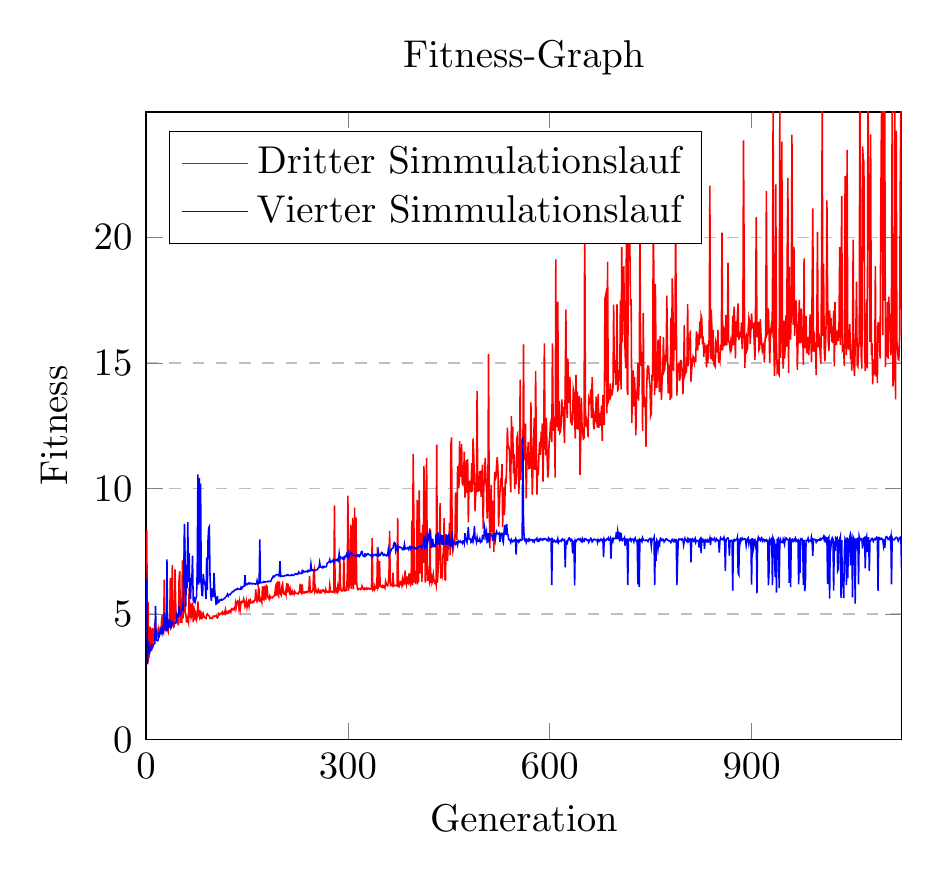
\begin{tikzpicture}[scale=1.4]
\begin{axis}[
    title={Fitness-Graph},
    xlabel={Generation},
    ylabel={Fitness},
    xmin=0, xmax=1123,
    ymin=0, ymax=25,
    xtick={0,300,600,900},
    ytick={0,5,10,15,20},
    legend pos=north west,
    ymajorgrids=true,
    grid style=dashed,
]

\addplot[
    color=red,
    mark=none,
    ]
    coordinates {
		(1,8.337641716003418)(2,4.0184645652771)(3,5.487634658813477)(4,3.268771171569824)(5,3.3982250690460205)(6,4.499021053314209)(7,3.691309928894043)(8,3.515028476715088)(9,4.444721698760986)(10,3.7522518634796143)(11,4.416717052459717)(12,4.221019744873047)(13,4.656446933746338)(14,4.452321529388428)(15,4.2899699211120605)(16,4.296048641204834)(17,4.185706615447998)(18,4.400793552398682)(19,4.207111358642578)(20,4.209735870361328)(21,4.4978742599487305)(22,4.218533992767334)(23,4.752462863922119)(24,4.955465316772461)(25,4.439781188964844)(26,4.3493852615356445)(27,6.367150783538818)(28,4.399297714233398)(29,4.336409568786621)(30,4.342099666595459)(31,4.4020256996154785)(32,4.515952110290527)(33,4.368217468261719)(34,4.791326522827148)(35,4.45461893081665)(36,6.443696022033691)(37,4.419928550720215)(38,5.808598518371582)(39,6.948536396026611)(40,4.520549297332764)(41,4.478343486785889)(42,4.533632755279541)(43,6.775493621826172)(44,5.4502081871032715)(45,4.674271583557129)(46,4.994293212890625)(47,4.611711502075195)(48,4.591427326202393)(49,6.427005290985107)(50,6.705092906951904)(51,4.635998725891113)(52,5.231718063354492)(53,4.6404242515563965)(54,7.138228416442871)(55,4.83296537399292)(56,5.4575300216674805)(57,8.198183059692383)(58,5.079111099243164)(59,5.0220746994018555)(60,4.698448181152344)(61,4.68707799911499)(62,4.85097074508667)(63,4.704654216766357)(64,6.040665149688721)(65,4.855485439300537)(66,5.410482883453369)(67,4.8824262619018555)(68,5.001476764678955)(69,5.468139171600342)(70,4.679938316345215)(71,5.3241658210754395)(72,4.756335735321045)(73,5.14747428894043)(74,4.917906761169434)(75,4.781447410583496)(76,4.917176723480225)(77,5.501983642578125)(78,5.0390305519104)(79,4.915684700012207)(80,5.1493611335754395)(81,4.827454090118408)(82,4.818329811096191)(83,5.000281810760498)(84,4.9070868492126465)(85,5.01362419128418)(86,4.908276081085205)(87,4.85512638092041)(88,4.851202964782715)(89,4.827971935272217)(90,4.951343059539795)(91,5.004500865936279)(92,4.960535526275635)(93,4.944637298583984)(94,4.923300266265869)(95,4.832083702087402)(96,4.853445529937744)(97,4.840818881988525)(98,4.823878765106201)(99,4.86625337600708)(100,4.92139196395874)(101,4.902008533477783)(102,4.914008617401123)(103,4.9282917976379395)(104,4.9483466148376465)(105,4.872841835021973)(106,4.846538066864014)(107,4.901675701141357)(108,5.014965057373047)(109,4.977746486663818)(110,5.01361608505249)(111,5.017216682434082)(112,5.0269775390625)(113,5.077807426452637)(114,4.990851402282715)(115,5.013479709625244)(116,5.076681137084961)(117,5.024285316467285)(118,5.172077655792236)(119,5.035671234130859)(120,5.077672481536865)(121,5.042375087738037)(122,5.095099925994873)(123,5.052812576293945)(124,5.150252819061279)(125,5.150534152984619)(126,5.077566146850586)(127,5.214122772216797)(128,5.196901798248291)(129,5.164315700531006)(130,5.227552890777588)(131,5.2450151443481445)(132,5.174229145050049)(133,5.4344987869262695)(134,5.295436382293701)(135,5.478116989135742)(136,5.527557849884033)(137,5.5007805824279785)(138,5.2363386154174805)(139,5.471573829650879)(140,5.216929912567139)(141,5.459837913513184)(142,5.496150970458984)(143,5.460948467254639)(144,5.491139888763428)(145,5.602490425109863)(146,5.509171485900879)(147,5.28665018081665)(148,5.3470048904418945)(149,5.5070905685424805)(150,5.271644115447998)(151,5.4166717529296875)(152,5.492286205291748)(153,5.319854259490967)(154,5.547508239746094)(155,5.576730728149414)(156,5.448465347290039)(157,5.455822467803955)(158,5.449313163757324)(159,5.506827354431152)(160,5.482302188873291)(161,5.550088405609131)(162,5.551332473754883)(163,5.984519958496094)(164,5.584130764007568)(165,5.491419792175293)(166,5.5435709953308105)(167,6.066195964813232)(168,5.98124361038208)(169,5.514509201049805)(170,5.510713577270508)(171,5.593795299530029)(172,5.482753276824951)(173,6.105553150177002)(174,5.609029293060303)(175,5.573231220245361)(176,6.12153434753418)(177,5.620379447937012)(178,5.6034255027771)(179,6.12676477432251)(180,6.093432426452637)(181,5.665706157684326)(182,5.667459011077881)(183,5.59725284576416)(184,5.7189412117004395)(185,5.645261287689209)(186,5.671420574188232)(187,5.666311740875244)(188,5.6499433517456055)(189,5.705088138580322)(190,5.703743934631348)(191,5.750663757324219)(192,5.96174430847168)(193,5.727972030639648)(194,6.212698459625244)(195,6.248234748840332)(196,5.763514041900635)(197,5.708507537841797)(198,6.303860187530518)(199,5.936214923858643)(200,5.7999587059021)(201,5.750758647918701)(202,6.127094268798828)(203,6.209222793579102)(204,5.8486833572387695)(205,5.795762538909912)(206,5.79394006729126)(207,5.8914947509765625)(208,5.774281978607178)(209,6.22984504699707)(210,5.854926109313965)(211,6.2078657150268555)(212,5.992016315460205)(213,5.8830885887146)(214,5.998076915740967)(215,5.783575057983398)(216,5.796772480010986)(217,5.919125080108643)(218,5.821643352508545)(219,5.865200519561768)(220,5.794439315795898)(221,5.899688243865967)(222,5.835334300994873)(223,5.820164680480957)(224,5.827912330627441)(225,5.819459438323975)(226,5.805851459503174)(227,5.873042583465576)(228,5.873746395111084)(229,6.211477279663086)(230,5.8588433265686035)(231,5.82452392578125)(232,6.179264068603516)(233,5.839381694793701)(234,5.849844932556152)(235,5.880352020263672)(236,5.848284721374512)(237,5.880436897277832)(238,5.861535549163818)(239,5.894623279571533)(240,5.868905067443848)(241,5.890384197235107)(242,6.002275466918945)(243,6.515683174133301)(244,5.878510475158691)(245,5.917879104614258)(246,5.879128932952881)(247,5.8981523513793945)(248,5.924780368804932)(249,6.6742777824401855)(250,6.779207706451416)(251,5.9349212646484375)(252,6.0362162590026855)(253,5.88839054107666)(254,5.852389812469482)(255,5.933241844177246)(256,5.981642723083496)(257,5.868082046508789)(258,5.849206924438477)(259,5.914815902709961)(260,5.854424476623535)(261,5.873373985290527)(262,5.9650559425354)(263,5.962552547454834)(264,5.912094593048096)(265,5.928625106811523)(266,5.866553783416748)(267,5.982507228851318)(268,5.880831241607666)(269,5.870488166809082)(270,5.895179271697998)(271,5.86417293548584)(272,5.861905574798584)(273,6.161482810974121)(274,5.94422721862793)(275,5.879997730255127)(276,5.875472068786621)(277,5.872368812561035)(278,5.908031463623047)(279,5.87587833404541)(280,9.331642150878906)(281,5.983882427215576)(282,5.896463871002197)(283,5.982696533203125)(284,5.898351669311523)(285,6.109954833984375)(286,5.924178123474121)(287,5.972482681274414)(288,7.226958751678467)(289,6.114979267120361)(290,5.927273273468018)(291,5.92030668258667)(292,5.923462390899658)(293,5.962270736694336)(294,7.198757648468018)(295,5.927533149719238)(296,5.928490161895752)(297,5.958340644836426)(298,5.953225612640381)(299,6.483359336853027)(300,9.712859153747559)(301,5.938929557800293)(302,6.169693470001221)(303,6.525606632232666)(304,8.560317039489746)(305,6.005934238433838)(306,6.646755695343018)(307,8.832021713256836)(308,5.9822468757629395)(309,6.478204250335693)(310,9.234922409057617)(311,6.176197528839111)(312,8.843140602111816)(313,6.284359455108643)(314,6.0345845222473145)(315,5.975447177886963)(316,6.0107550621032715)(317,6.008316993713379)(318,6.0171027183532715)(319,5.976761341094971)(320,5.986345291137695)(321,6.1153364181518555)(322,6.039125919342041)(323,6.004708290100098)(324,5.9759697914123535)(325,6.032904148101807)(326,5.998688697814941)(327,5.985610008239746)(328,6.038085460662842)(329,5.995763301849365)(330,6.0096049308776855)(331,6.030975341796875)(332,5.996053695678711)(333,5.999397277832031)(334,6.007864952087402)(335,5.998436450958252)(336,8.02116584777832)(337,5.984915733337402)(338,6.032752990722656)(339,5.966975212097168)(340,6.1228928565979)(341,6.0206732749938965)(342,6.046128273010254)(343,6.040995121002197)(344,7.668386936187744)(345,6.052603721618652)(346,6.111850261688232)(347,7.120563507080078)(348,6.104676723480225)(349,6.097665309906006)(350,6.0761823654174805)(351,6.128442764282227)(352,6.0666704177856445)(353,6.116689205169678)(354,6.087969779968262)(355,6.0356669425964355)(356,6.304139137268066)(357,6.2051920890808105)(358,6.147895812988281)(359,6.127424716949463)(360,6.245117664337158)(361,6.601839065551758)(362,8.316102027893066)(363,6.13275146484375)(364,6.138503551483154)(365,6.1789984703063965)(366,6.142375469207764)(367,6.64583683013916)(368,6.1160969734191895)(369,6.1396965980529785)(370,6.147129058837891)(371,6.137656211853027)(372,6.132750511169434)(373,6.122639179229736)(374,8.823402404785156)(375,6.148833751678467)(376,6.093331813812256)(377,6.163819313049316)(378,6.296420097351074)(379,6.284384250640869)(380,6.1558732986450195)(381,6.391622066497803)(382,6.2254638671875)(383,6.348618507385254)(384,6.173797607421875)(385,6.742833137512207)(386,6.2859673500061035)(387,6.17417573928833)(388,6.4993414878845215)(389,6.259109020233154)(390,6.219954490661621)(391,6.631834506988525)(392,6.298503875732422)(393,6.202667713165283)(394,6.358299732208252)(395,8.720865249633789)(396,6.144345760345459)(397,11.381012916564941)(398,8.887557983398438)(399,6.256819248199463)(400,6.458901405334473)(401,6.191874980926514)(402,6.737107276916504)(403,9.544281959533691)(404,6.266107559204102)(405,6.316109657287598)(406,9.928303718566895)(407,6.791256427764893)(408,6.615273952484131)(409,8.236763000488281)(410,6.283973693847656)(411,8.567084312438965)(412,7.043710231781006)(413,10.895868301391602)(414,8.543363571166992)(415,6.257015228271484)(416,9.55417537689209)(417,11.219818115234375)(418,6.32145881652832)(419,6.6287841796875)(420,6.460313320159912)(421,6.323060035705566)(422,8.40581226348877)(423,6.231586456298828)(424,6.614081382751465)(425,6.247429847717285)(426,6.335134506225586)(427,6.563512802124023)(428,6.3099188804626465)(429,6.247495651245117)(430,6.307552814483643)(431,6.177356719970703)(432,11.753419876098633)(433,6.245326995849609)(434,6.716487884521484)(435,7.1390862464904785)(436,7.943373680114746)(437,9.416289329528809)(438,6.413801670074463)(439,6.742499828338623)(440,6.591031551361084)(441,7.2711358070373535)(442,7.491066932678223)(443,8.823219299316406)(444,6.385529041290283)(445,6.361673355102539)(446,7.923859596252441)(447,7.864811897277832)(448,7.124953746795654)(449,7.718211650848389)(450,7.679666519165039)(451,8.631969451904297)(452,7.343308448791504)(453,11.720011711120605)(454,12.033319473266602)(455,7.852997779846191)(456,7.497190475463867)(457,7.639498710632324)(458,8.003934860229492)(459,7.76599645614624)(460,9.8501615524292)(461,9.07846450805664)(462,7.948515892028809)(463,10.895465850830078)(464,10.560994148254395)(465,10.025009155273438)(466,11.8927640914917)(467,10.46627426147461)(468,10.622767448425293)(469,11.773374557495117)(470,10.187896728515625)(471,10.150663375854492)(472,10.495702743530273)(473,11.472249031066895)(474,9.635607719421387)(475,10.105985641479492)(476,11.132173538208008)(477,9.817951202392578)(478,11.173310279846191)(479,8.649094581604004)(480,10.314362525939941)(481,9.881608963012695)(482,10.100751876831055)(483,9.85138988494873)(484,11.014360427856445)(485,9.881974220275879)(486,11.997859001159668)(487,11.353585243225098)(488,10.389106750488281)(489,9.08838176727295)(490,9.75267505645752)(491,9.946430206298828)(492,13.893165588378906)(493,9.872443199157715)(494,10.507830619812012)(495,9.887391090393066)(496,10.665759086608887)(497,10.676892280578613)(498,9.665061950683594)(499,10.229191780090332)(500,10.956282615661621)(501,8.406309127807617)(502,10.094558715820312)(503,10.308785438537598)(504,11.219680786132812)(505,10.5119047164917)(506,9.899886131286621)(507,8.799631118774414)(508,9.473828315734863)(509,15.350695610046387)(510,9.605722427368164)(511,7.621309280395508)(512,9.557476997375488)(513,10.14732837677002)(514,8.250448226928711)(515,8.471990585327148)(516,9.514994621276855)(517,7.46364164352417)(518,10.662060737609863)(519,10.36086654663086)(520,10.430702209472656)(521,10.962834358215332)(522,11.244498252868652)(523,10.808643341064453)(524,8.48244571685791)(525,9.197649955749512)(526,9.881793975830078)(527,10.414412498474121)(528,10.12694263458252)(529,10.974458694458008)(530,8.474931716918945)(531,10.041888236999512)(532,8.948553085327148)(533,9.125262260437012)(534,10.388158798217773)(535,10.203831672668457)(536,10.96680736541748)(537,12.421212196350098)(538,11.699240684509277)(539,11.678580284118652)(540,11.504353523254395)(541,10.633057594299316)(542,9.843705177307129)(543,12.880253791809082)(544,11.194149017333984)(545,12.46596908569336)(546,10.601951599121094)(547,11.37965202331543)(548,9.988120079040527)(549,10.813209533691406)(550,10.16409969329834)(551,12.00001335144043)(552,12.108620643615723)(553,11.104337692260742)(554,9.78674602508545)(555,10.62694263458252)(556,14.337990760803223)(557,10.332179069519043)(558,11.839805603027344)(559,11.917978286743164)(560,11.049240112304688)(561,15.740185737609863)(562,11.1229248046875)(563,12.266275405883789)(564,12.582237243652344)(565,9.605339050292969)(566,11.057835578918457)(567,11.177360534667969)(568,11.845305442810059)(569,10.764891624450684)(570,10.979349136352539)(571,10.795829772949219)(572,13.429532051086426)(573,11.738264083862305)(574,9.75357437133789)(575,10.705971717834473)(576,11.803427696228027)(577,12.809099197387695)(578,10.741613388061523)(579,14.672120094299316)(580,11.979580879211426)(581,9.761622428894043)(582,10.895533561706543)(583,10.528770446777344)(584,11.372077941894531)(585,11.856425285339355)(586,11.337483406066895)(587,12.009407043457031)(588,11.851785659790039)(589,12.593582153320312)(590,10.276772499084473)(591,12.147674560546875)(592,15.78609561920166)(593,12.211490631103516)(594,11.318446159362793)(595,12.816551208496094)(596,11.380187034606934)(597,10.435059547424316)(598,10.610873222351074)(599,11.812215805053711)(600,12.035940170288086)(601,12.553868293762207)(602,12.393935203552246)(603,11.84714412689209)(604,15.786105155944824)(605,12.765387535095215)(606,12.295071601867676)(607,12.859504699707031)(608,10.435474395751953)(609,19.130868911743164)(610,12.44633960723877)(611,12.881175994873047)(612,17.449438095092773)(613,12.29190444946289)(614,13.494592666625977)(615,12.221550941467285)(616,12.269068717956543)(617,12.572835922241211)(618,13.546876907348633)(619,12.879454612731934)(620,13.24911880493164)(621,12.445784568786621)(622,11.809772491455078)(623,14.234458923339844)(624,17.128246307373047)(625,13.2974853515625)(626,12.817977905273438)(627,15.173672676086426)(628,13.740854263305664)(629,13.403345108032227)(630,14.448265075683594)(631,12.728260040283203)(632,12.800707817077637)(633,12.521868705749512)(634,12.814543724060059)(635,13.993440628051758)(636,13.854349136352539)(637,12.805520057678223)(638,11.987524032592773)(639,14.524024963378906)(640,12.37874984741211)(641,13.873872756958008)(642,12.348306655883789)(643,13.390318870544434)(644,13.687944412231445)(645,10.546338081359863)(646,11.83608341217041)(647,13.609733581542969)(648,12.521965980529785)(649,12.216780662536621)(650,11.982443809509277)(651,12.016454696655273)(652,21.52263641357422)(653,13.191690444946289)(654,12.452725410461426)(655,12.70211410522461)(656,12.569183349609375)(657,12.041511535644531)(658,13.545388221740723)(659,13.410118103027344)(660,13.495165824890137)(661,13.946102142333984)(662,12.811720848083496)(663,14.438326835632324)(664,13.403158187866211)(665,12.551753044128418)(666,12.355093002319336)(667,12.821682929992676)(668,12.655981063842773)(669,13.667499542236328)(670,12.657811164855957)(671,12.42665958404541)(672,13.76744270324707)(673,12.414911270141602)(674,13.008515357971191)(675,12.49912166595459)(676,12.758234024047852)(677,13.300078392028809)(678,11.895895004272461)(679,13.732287406921387)(680,13.504582405090332)(681,12.529562950134277)(682,17.555883407592773)(683,17.68995475769043)(684,14.831342697143555)(685,12.989914894104004)(686,19.037742614746094)(687,13.459678649902344)(688,13.551830291748047)(689,13.613574981689453)(690,14.185062408447266)(691,13.723258018493652)(692,13.848760604858398)(693,13.796547889709473)(694,14.04462718963623)(695,17.321630477905273)(696,14.599445343017578)(697,15.112615585327148)(698,14.118462562561035)(699,14.617371559143066)(700,17.33296012878418)(701,13.91675853729248)(702,13.95689582824707)(703,14.722501754760742)(704,14.28674030303955)(705,17.492633819580078)(706,13.935425758361816)(707,19.61759376525879)(708,15.820049285888672)(709,18.797155380249023)(710,18.81688690185547)(711,16.90828514099121)(712,15.408597946166992)(713,14.789905548095703)(714,20.62088966369629)(715,13.967487335205078)(716,13.732381820678711)(717,22.253368377685547)(718,19.499269485473633)(719,19.903200149536133)(720,17.294567108154297)(721,17.54410171508789)(722,12.61589527130127)(723,14.141013145446777)(724,14.707757949829102)(725,13.264033317565918)(726,14.44320011138916)(727,13.690934181213379)(728,12.116867065429688)(729,13.713753700256348)(730,13.896805763244629)(731,15.007745742797852)(732,13.501983642578125)(733,14.37324333190918)(734,20.343257904052734)(735,15.989080429077148)(736,14.888601303100586)(737,15.439072608947754)(738,12.293525695800781)(739,16.998727798461914)(740,13.735053062438965)(741,13.23335075378418)(742,13.625689506530762)(743,11.655915260314941)(744,13.899579048156738)(745,14.762616157531738)(746,14.875219345092773)(747,14.861174583435059)(748,14.322209358215332)(749,14.117695808410645)(750,12.89001178741455)(751,12.984481811523438)(752,14.529468536376953)(753,14.294950485229492)(754,22.223079681396484)(755,16.583982467651367)(756,13.724838256835938)(757,18.148401260375977)(758,15.149996757507324)(759,14.014505386352539)(760,14.521781921386719)(761,15.939119338989258)(762,14.653594017028809)(763,13.845129013061523)(764,16.07008934020996)(765,14.518941879272461)(766,13.532553672790527)(767,14.281267166137695)(768,14.717241287231445)(769,16.029455184936523)(770,14.687213897705078)(771,14.769811630249023)(772,15.330819129943848)(773,15.054826736450195)(774,17.6823787689209)(775,15.699328422546387)(776,13.793977737426758)(777,14.927489280700684)(778,14.742931365966797)(779,13.517706871032715)(780,16.80513572692871)(781,13.604636192321777)(782,18.37032127380371)(783,17.528095245361328)(784,14.681078910827637)(785,16.149690628051758)(786,15.51143741607666)(787,20.556896209716797)(788,17.392044067382812)(789,13.706050872802734)(790,14.83946704864502)(791,14.939262390136719)(792,14.987822532653809)(793,14.291227340698242)(794,14.504085540771484)(795,15.12553882598877)(796,14.776484489440918)(797,14.728206634521484)(798,13.762613296508789)(799,14.785649299621582)(800,16.511987686157227)(801,14.540836334228516)(802,14.63330078125)(803,14.633193969726562)(804,15.093789100646973)(805,17.357240676879883)(806,14.875019073486328)(807,15.962015151977539)(808,15.672727584838867)(809,16.294437408447266)(810,14.258255958557129)(811,14.715581893920898)(812,15.095990180969238)(813,15.254608154296875)(814,15.18607234954834)(815,15.010178565979004)(816,15.167162895202637)(817,15.112454414367676)(818,16.263046264648438)(819,15.883532524108887)(820,15.50489330291748)(821,16.155378341674805)(822,15.71647834777832)(823,16.66037368774414)(824,15.976778030395508)(825,16.883071899414062)(826,16.765644073486328)(827,15.74810791015625)(828,16.062015533447266)(829,15.246615409851074)(830,15.80415153503418)(831,15.419637680053711)(832,15.697975158691406)(833,14.831314086914062)(834,15.736610412597656)(835,15.004059791564941)(836,15.752942085266113)(837,15.96069622039795)(838,22.060712814331055)(839,15.150398254394531)(840,17.129343032836914)(841,16.40666961669922)(842,15.075349807739258)(843,16.32088851928711)(844,14.958089828491211)(845,14.9000244140625)(846,14.851774215698242)(847,15.806025505065918)(848,15.660978317260742)(849,15.412995338439941)(850,16.32326316833496)(851,15.011798858642578)(852,15.260771751403809)(853,15.115198135375977)(854,15.728132247924805)(855,15.504555702209473)(856,20.19776153564453)(857,15.506054878234863)(858,16.488473892211914)(859,16.256256103515625)(860,15.676587104797363)(861,16.170103073120117)(862,16.91322898864746)(863,15.698938369750977)(864,16.11931037902832)(865,18.994735717773438)(866,15.87725830078125)(867,15.799551963806152)(868,15.558858871459961)(869,15.82440185546875)(870,15.581077575683594)(871,15.73464584350586)(872,16.882343292236328)(873,15.711263656616211)(874,17.243715286254883)(875,16.628511428833008)(876,15.181331634521484)(877,16.65973663330078)(878,16.034839630126953)(879,16.98039436340332)(880,17.37567901611328)(881,15.9118070602417)(882,16.120250701904297)(883,16.18462562561035)(884,16.087453842163086)(885,16.62026023864746)(886,15.55885124206543)(887,16.049230575561523)(888,23.864830017089844)(889,19.156200408935547)(890,14.80601978302002)(891,15.977394104003906)(892,16.064834594726562)(893,15.493753433227539)(894,15.581564903259277)(895,16.36583137512207)(896,16.79546356201172)(897,16.61677360534668)(898,15.76761531829834)(899,16.394628524780273)(900,16.977102279663086)(901,16.438974380493164)(902,16.48591423034668)(903,16.530338287353516)(904,15.737847328186035)(905,15.128265380859375)(906,17.505599975585938)(907,20.812477111816406)(908,16.02594757080078)(909,16.305082321166992)(910,16.6348819732666)(911,15.513566970825195)(912,15.591757774353027)(913,16.74704933166504)(914,16.16061782836914)(915,15.778461456298828)(916,15.487920761108398)(917,15.615060806274414)(918,15.803433418273926)(919,15.012228965759277)(920,15.8975248336792)(921,16.16417121887207)(922,21.85502052307129)(923,16.15078353881836)(924,16.235706329345703)(925,17.170333862304688)(926,16.249528884887695)(927,14.988199234008789)(928,16.17699432373047)(929,16.412704467773438)(930,16.273685455322266)(931,17.264623641967773)(932,25.13562774658203)(933,15.971452713012695)(934,14.479177474975586)(935,15.294669151306152)(936,22.110733032226562)(937,15.804564476013184)(938,14.758651733398438)(939,14.907369613647461)(940,14.581833839416504)(941,14.527998924255371)(942,25.187713623046875)(943,15.209573745727539)(944,17.248685836791992)(945,23.81985855102539)(946,15.780562400817871)(947,14.773159980773926)(948,16.69244956970215)(949,15.171592712402344)(950,15.6187162399292)(951,16.89236068725586)(952,15.649706840515137)(953,19.54820442199707)(954,22.376176834106445)(955,14.611660957336426)(956,18.8342342376709)(957,16.502891540527344)(958,15.929694175720215)(959,17.11600112915039)(960,24.094758987426758)(961,17.363788604736328)(962,16.521991729736328)(963,19.622190475463867)(964,16.085241317749023)(965,16.84160804748535)(966,17.492162704467773)(967,16.794710159301758)(968,14.728360176086426)(969,15.77258014678955)(970,16.52113151550293)(971,17.51325035095215)(972,15.815454483032227)(973,15.812150001525879)(974,17.163042068481445)(975,15.810914039611816)(976,16.239498138427734)(977,14.924250602722168)(978,19.165233612060547)(979,15.592377662658691)(980,16.01264762878418)(981,16.868011474609375)(982,15.385257720947266)(983,16.040607452392578)(984,15.84909725189209)(985,15.319718360900879)(986,15.967841148376465)(987,16.934375762939453)(988,16.493946075439453)(989,15.027729988098145)(990,18.012676239013672)(991,21.15669822692871)(992,15.453804969787598)(993,16.253681182861328)(994,15.443765640258789)(995,15.82069206237793)(996,14.520870208740234)(997,16.717180252075195)(998,20.227909088134766)(999,15.62635326385498)(1000,16.184709548950195)(1001,15.917961120605469)(1002,15.361420631408691)(1003,14.980744361877441)(1004,18.886186599731445)(1005,25.208202362060547)(1006,16.066316604614258)(1007,18.95525360107422)(1008,15.587867736816406)(1009,15.067076683044434)(1010,15.716431617736816)(1011,16.813112258911133)(1012,21.473995208740234)(1013,17.75836944580078)(1014,15.80489730834961)(1015,15.477217674255371)(1016,17.09370994567871)(1017,16.168598175048828)(1018,16.80103302001953)(1019,15.886938095092773)(1020,15.85312271118164)(1021,16.075456619262695)(1022,17.087377548217773)(1023,14.866348266601562)(1024,17.425495147705078)(1025,15.918926239013672)(1026,15.710957527160645)(1027,16.085914611816406)(1028,16.297203063964844)(1029,15.87238883972168)(1030,16.622764587402344)(1031,19.620500564575195)(1032,15.72467041015625)(1033,17.50066375732422)(1034,21.656085968017578)(1035,15.555668830871582)(1036,15.631111145019531)(1037,15.376730918884277)(1038,14.887652397155762)(1039,22.442041397094727)(1040,16.5877685546875)(1041,15.313490867614746)(1042,23.49057388305664)(1043,15.742307662963867)(1044,15.86677074432373)(1045,15.527106285095215)(1046,16.5620174407959)(1047,15.290735244750977)(1048,15.37162971496582)(1049,14.696459770202637)(1050,15.688087463378906)(1051,19.91805648803711)(1052,14.920710563659668)(1053,14.48491096496582)(1054,15.610963821411133)(1055,16.253137588500977)(1056,18.24379539489746)(1057,14.919161796569824)(1058,14.861735343933105)(1059,15.537409782409668)(1060,15.879759788513184)(1061,27.55990219116211)(1062,16.44008445739746)(1063,15.266425132751465)(1064,14.779086112976074)(1065,23.623388290405273)(1066,23.168048858642578)(1067,22.986120223999023)(1068,15.490964889526367)(1069,14.690497398376465)(1070,16.42139434814453)(1071,17.53693389892578)(1072,14.785414695739746)(1073,26.3134822845459)(1074,22.281267166137695)(1075,21.208995819091797)(1076,15.837249755859375)(1077,24.108417510986328)(1078,15.312273025512695)(1079,15.781268119812012)(1080,14.145896911621094)(1081,15.138900756835938)(1082,14.557621002197266)(1083,14.607288360595703)(1084,18.86101722717285)(1085,14.459778785705566)(1086,15.82988452911377)(1087,14.20572566986084)(1088,16.62837791442871)(1089,15.996018409729004)(1090,16.60219383239746)(1091,15.17453670501709)(1092,20.72237777709961)(1093,24.72115707397461)(1094,25.543710708618164)(1095,16.116262435913086)(1096,25.163047790527344)(1097,17.4805850982666)(1098,25.24859619140625)(1099,14.8487548828125)(1100,16.140615463256836)(1101,15.241332054138184)(1102,17.42087173461914)(1103,15.164253234863281)(1104,17.647579193115234)(1105,16.55990219116211)(1106,16.448610305786133)(1107,15.300239562988281)(1108,17.796459197998047)(1109,25.461397171020508)(1110,14.065865516662598)(1111,14.337145805358887)(1112,15.31286907196045)(1113,25.27859115600586)(1114,13.556527137756348)(1115,24.248794555664062)(1116,15.89082145690918)(1117,15.494329452514648)(1118,15.14848518371582)(1119,15.124610900878906)(1120,16.048625946044922)(1121,22.123979568481445)(1122,25.5994873046875)(1123,16.12203598022461)
	};
    \addlegendentry{Dritter Simmulationslauf}

    \addplot[
        color=blue,
        mark=none,
        ]
        coordinates {
(1,6.396632194519043)(2,3.001333236694336)(3,3.8736047744750977)(4,3.850943088531494)(5,3.43033766746521)(6,3.633312463760376)(7,3.600954055786133)(8,3.7289016246795654)(9,3.647129535675049)(10,3.6877758502960205)(11,3.770575523376465)(12,3.821573257446289)(13,3.830167055130005)(14,5.329158782958984)(15,3.9852652549743652)(16,3.9554460048675537)(17,3.9389240741729736)(18,3.9635047912597656)(19,4.210161209106445)(20,4.152338027954102)(21,4.2883524894714355)(22,4.388443946838379)(23,4.27398681640625)(24,4.388275623321533)(25,4.2364020347595215)(26,4.355759620666504)(27,5.056122779846191)(28,4.522096633911133)(29,4.397518157958984)(30,4.3791022300720215)(31,7.178400039672852)(32,4.417032241821289)(33,4.4969072341918945)(34,4.4964518547058105)(35,4.745449542999268)(36,4.724573612213135)(37,4.480184078216553)(38,4.5808281898498535)(39,4.661709785461426)(40,4.610383033752441)(41,4.6147308349609375)(42,4.617713451385498)(43,4.642808437347412)(44,4.644167900085449)(45,4.719897270202637)(46,4.967432975769043)(47,4.906210422515869)(48,4.932036876678467)(49,5.311508655548096)(50,5.050005912780762)(51,4.9908270835876465)(52,5.0829362869262695)(53,5.143371105194092)(54,5.303469181060791)(55,5.129563808441162)(56,6.494692802429199)(57,8.596389770507812)(58,7.2329630851745605)(59,5.29355001449585)(60,6.963648319244385)(61,6.033735752105713)(62,8.659967422485352)(63,6.286695957183838)(64,7.422773361206055)(65,5.789124011993408)(66,5.600589752197266)(67,6.365304470062256)(68,6.331460952758789)(69,7.328947067260742)(70,5.55446195602417)(71,5.5057902336120605)(72,5.598186492919922)(73,5.496506690979004)(74,5.61646032333374)(75,5.7104082107543945)(76,6.778139591217041)(77,10.566896438598633)(78,6.169734477996826)(79,10.417387008666992)(80,6.250974655151367)(81,10.199295043945312)(82,6.187450408935547)(83,5.758698463439941)(84,5.7421793937683105)(85,6.600430488586426)(86,6.320876598358154)(87,6.217523574829102)(88,6.1347174644470215)(89,5.596717357635498)(90,7.2447333335876465)(91,5.9580535888671875)(92,7.928491592407227)(93,8.421905517578125)(94,8.47918701171875)(95,6.540931224822998)(96,5.819090366363525)(97,5.530434608459473)(98,6.021536827087402)(99,5.7213358879089355)(100,5.710623741149902)(101,6.642415523529053)(102,5.954791069030762)(103,5.649866580963135)(104,5.392682075500488)(105,5.4137725830078125)(106,5.71885871887207)(107,5.46360969543457)(108,5.483486652374268)(109,5.501834869384766)(110,5.570995807647705)(111,5.559449672698975)(112,5.5817389488220215)(113,5.557476043701172)(114,5.578113555908203)(115,5.589656352996826)(116,5.622227668762207)(117,5.629795551300049)(118,5.674586772918701)(119,5.700262069702148)(120,5.728970527648926)(121,5.788483142852783)(122,5.721715450286865)(123,5.786418437957764)(124,5.785367012023926)(125,5.770878791809082)(126,5.818362712860107)(127,5.844974040985107)(128,5.880740165710449)(129,5.8875555992126465)(130,5.8948211669921875)(131,5.938600540161133)(132,5.956265926361084)(133,5.97654914855957)(134,5.969476699829102)(135,5.999143123626709)(136,6.020541191101074)(137,5.990149974822998)(138,5.993375301361084)(139,5.994913578033447)(140,5.992498397827148)(141,6.063217639923096)(142,6.005139350891113)(143,6.04948091506958)(144,6.099338531494141)(145,6.1066389083862305)(146,6.121620178222656)(147,6.544992446899414)(148,6.168539524078369)(149,6.1997785568237305)(150,6.175652980804443)(151,6.208289623260498)(152,6.203786849975586)(153,6.242534160614014)(154,6.2010602951049805)(155,6.224192142486572)(156,6.228313446044922)(157,6.205789566040039)(158,6.198624610900879)(159,6.221116065979004)(160,6.215169429779053)(161,6.20831823348999)(162,6.191043376922607)(163,6.196863651275635)(164,6.21624755859375)(165,6.335719585418701)(166,6.196800708770752)(167,6.22822904586792)(168,6.224162578582764)(169,7.974237442016602)(170,6.251083850860596)(171,6.258689880371094)(172,6.249848365783691)(173,6.259819984436035)(174,6.264815330505371)(175,6.296242713928223)(176,6.276998519897461)(177,6.277915954589844)(178,6.292148590087891)(179,6.28985071182251)(180,6.294747829437256)(181,6.2840375900268555)(182,6.309423923492432)(183,6.30316162109375)(184,6.306175231933594)(185,6.299269199371338)(186,6.346637725830078)(187,6.4241156578063965)(188,6.434574127197266)(189,6.507828712463379)(190,6.482964992523193)(191,6.505818843841553)(192,6.541637420654297)(193,6.548863410949707)(194,6.574493408203125)(195,6.570940971374512)(196,6.568523406982422)(197,6.524694919586182)(198,6.526160717010498)(199,7.106166839599609)(200,6.505735874176025)(201,6.52601432800293)(202,6.511237621307373)(203,6.505593299865723)(204,6.507566452026367)(205,6.511762619018555)(206,6.539295196533203)(207,6.5309953689575195)(208,6.5305681228637695)(209,6.55291223526001)(210,6.567346096038818)(211,6.539247512817383)(212,6.556546211242676)(213,6.54171895980835)(214,6.531126022338867)(215,6.549560070037842)(216,6.556812286376953)(217,6.566710948944092)(218,6.5386176109313965)(219,6.537637710571289)(220,6.5635881423950195)(221,6.592563152313232)(222,6.6052350997924805)(223,6.580439567565918)(224,6.597496032714844)(225,6.583973407745361)(226,6.617846965789795)(227,6.675002098083496)(228,6.616209030151367)(229,6.618345260620117)(230,6.616164684295654)(231,6.615274429321289)(232,6.7203874588012695)(233,6.664018630981445)(234,6.710312366485596)(235,6.679061412811279)(236,6.685791492462158)(237,6.681613445281982)(238,6.707733154296875)(239,6.7114763259887695)(240,6.682830810546875)(241,6.738099575042725)(242,6.709308624267578)(243,6.729803562164307)(244,6.722880840301514)(245,6.989043712615967)(246,6.7517476081848145)(247,6.736011028289795)(248,6.76029634475708)(249,6.744821071624756)(250,6.748688697814941)(251,6.721714973449707)(252,6.747113227844238)(253,6.762603282928467)(254,6.767137050628662)(255,6.777532577514648)(256,6.847316265106201)(257,6.850129127502441)(258,7.047654628753662)(259,6.884122371673584)(260,6.864641189575195)(261,6.86788272857666)(262,6.847459316253662)(263,6.89778470993042)(264,6.861443519592285)(265,6.893421649932861)(266,6.8808770179748535)(267,6.876903533935547)(268,6.8848114013671875)(269,7.015260696411133)(270,7.0434112548828125)(271,7.060929298400879)(272,7.076031684875488)(273,7.170254707336426)(274,7.054446697235107)(275,7.072078227996826)(276,7.102310657501221)(277,7.0928544998168945)(278,7.1528496742248535)(279,7.050770282745361)(280,7.127933979034424)(281,7.161865234375)(282,7.140349864959717)(283,7.165855884552002)(284,7.130743026733398)(285,7.188291549682617)(286,7.138206958770752)(287,7.408021926879883)(288,7.186578750610352)(289,7.267542839050293)(290,7.248281002044678)(291,7.259799480438232)(292,7.1969780921936035)(293,7.189865589141846)(294,7.255656719207764)(295,7.2133378982543945)(296,7.3061137199401855)(297,7.297480583190918)(298,7.384835720062256)(299,7.306496620178223)(300,7.259911060333252)(301,7.416697025299072)(302,7.290411472320557)(303,7.356680393218994)(304,7.38083553314209)(305,7.440270900726318)(306,7.422536849975586)(307,7.356286525726318)(308,7.325638294219971)(309,7.324927806854248)(310,7.323848247528076)(311,7.315363883972168)(312,7.341644763946533)(313,7.305680274963379)(314,7.303008079528809)(315,7.3622941970825195)(316,7.3503947257995605)(317,7.291415214538574)(318,7.332216739654541)(319,7.394679069519043)(320,7.48163366317749)(321,7.488402366638184)(322,7.3510518074035645)(323,7.31119966506958)(324,7.296233177185059)(325,7.369017601013184)(326,7.322159767150879)(327,7.383780002593994)(328,7.357069969177246)(329,7.387874126434326)(330,7.402122497558594)(331,7.376653671264648)(332,7.357135772705078)(333,7.358922958374023)(334,7.332411766052246)(335,7.3016676902771)(336,7.373437881469727)(337,7.2910380363464355)(338,7.341487407684326)(339,7.370055675506592)(340,7.377647876739502)(341,7.349050045013428)(342,7.361086368560791)(343,7.328634262084961)(344,7.359013557434082)(345,7.502194404602051)(346,7.330362319946289)(347,7.363345623016357)(348,7.343679428100586)(349,7.397828102111816)(350,7.454980850219727)(351,7.4462127685546875)(352,7.365783214569092)(353,7.34315824508667)(354,7.380013942718506)(355,7.352025508880615)(356,7.347074508666992)(357,7.323983669281006)(358,7.362630367279053)(359,7.345525741577148)(360,7.555161952972412)(361,7.322134017944336)(362,7.375275135040283)(363,7.523791313171387)(364,7.518813133239746)(365,7.610363006591797)(366,7.610660552978516)(367,7.634109020233154)(368,7.78782844543457)(369,7.848050594329834)(370,7.821678638458252)(371,7.531856536865234)(372,7.654134750366211)(373,7.7317728996276855)(374,7.530677318572998)(375,7.603333950042725)(376,7.681437969207764)(377,7.67332124710083)(378,7.660177230834961)(379,7.636366367340088)(380,7.641848564147949)(381,7.568715572357178)(382,7.562463760375977)(383,7.628767967224121)(384,7.7813262939453125)(385,7.599277019500732)(386,7.6270432472229)(387,7.607664108276367)(388,7.621081829071045)(389,7.645027160644531)(390,7.582215309143066)(391,7.6502532958984375)(392,7.687467098236084)(393,7.59545373916626)(394,7.6519598960876465)(395,7.679172515869141)(396,7.640838623046875)(397,7.652908802032471)(398,7.6563720703125)(399,7.647704124450684)(400,7.594714164733887)(401,7.622509002685547)(402,7.593861103057861)(403,7.622450351715088)(404,7.638613224029541)(405,7.67943000793457)(406,7.675662994384766)(407,7.702998161315918)(408,7.690145015716553)(409,7.728112697601318)(410,7.6418232917785645)(411,7.722462177276611)(412,7.787763595581055)(413,8.11871337890625)(414,7.766735553741455)(415,7.934110164642334)(416,7.673730850219727)(417,7.634751796722412)(418,8.088367462158203)(419,7.927576541900635)(420,8.093557357788086)(421,8.243780136108398)(422,8.072569847106934)(423,8.16254711151123)(424,7.66087007522583)(425,7.676560401916504)(426,8.004792213439941)(427,7.701590061187744)(428,7.691318511962891)(429,7.746891975402832)(430,7.713208198547363)(431,8.140640258789062)(432,8.118642807006836)(433,7.744028568267822)(434,8.252988815307617)(435,7.9022417068481445)(436,7.790460586547852)(437,7.913698196411133)(438,8.13671875)(439,8.102741241455078)(440,7.748414039611816)(441,8.142034530639648)(442,7.774231433868408)(443,7.775013446807861)(444,7.785923957824707)(445,7.8934760093688965)(446,8.18191909790039)(447,7.765657901763916)(448,8.146484375)(449,7.739920139312744)(450,8.204678535461426)(451,7.791461944580078)(452,7.755471229553223)(453,7.886122226715088)(454,7.782324314117432)(455,8.29997730255127)(456,7.7619709968566895)(457,7.880014419555664)(458,7.842087268829346)(459,7.819581985473633)(460,7.7829413414001465)(461,7.854148864746094)(462,7.874602794647217)(463,7.756472110748291)(464,7.900981903076172)(465,7.854604244232178)(466,7.869883060455322)(467,7.910641193389893)(468,7.859504699707031)(469,7.875661849975586)(470,7.823517799377441)(471,7.909857273101807)(472,7.920329570770264)(473,7.818001747131348)(474,8.222306251525879)(475,7.996851921081543)(476,7.928771495819092)(477,7.858162879943848)(478,8.112903594970703)(479,8.475604057312012)(480,7.999389171600342)(481,8.006246566772461)(482,7.987368583679199)(483,7.860781192779541)(484,7.899785995483398)(485,8.01423168182373)(486,7.886743545532227)(487,8.016281127929688)(488,8.498000144958496)(489,8.014429092407227)(490,8.000265121459961)(491,7.878180503845215)(492,8.05057430267334)(493,7.900153160095215)(494,7.910809516906738)(495,7.906049728393555)(496,7.988012313842773)(497,7.855768203735352)(498,7.880953788757324)(499,7.885415554046631)(500,8.099541664123535)(501,8.055842399597168)(502,8.019648551940918)(503,8.45467758178711)(504,8.28724479675293)(505,8.097996711730957)(506,8.254386901855469)(507,7.865882873535156)(508,7.891499996185303)(509,8.221877098083496)(510,7.957207679748535)(511,8.1810302734375)(512,8.184948921203613)(513,8.149137496948242)(514,8.174627304077148)(515,7.943971157073975)(516,7.955431938171387)(517,8.188191413879395)(518,8.19543743133545)(519,7.959256649017334)(520,8.161808013916016)(521,8.280325889587402)(522,8.199650764465332)(523,8.206120491027832)(524,8.187775611877441)(525,8.221880912780762)(526,7.875624179840088)(527,8.188826560974121)(528,8.209234237670898)(529,8.214361190795898)(530,7.934185981750488)(531,7.851109027862549)(532,8.240472793579102)(533,8.5521240234375)(534,8.19446086883545)(535,8.181608200073242)(536,8.593331336975098)(537,8.186378479003906)(538,8.150782585144043)(539,7.971808910369873)(540,7.96623420715332)(541,7.941717147827148)(542,7.852099418640137)(543,7.966763496398926)(544,7.9108428955078125)(545,7.884254455566406)(546,7.916353702545166)(547,7.941505432128906)(548,7.912683486938477)(549,7.978543758392334)(550,7.369458198547363)(551,7.936820983886719)(552,7.9001593589782715)(553,7.930784702301025)(554,7.864962577819824)(555,7.909679889678955)(556,7.965603828430176)(557,7.935959815979004)(558,7.947145938873291)(559,7.9652628898620605)(560,12.056096076965332)(561,8.704976081848145)(562,7.972678184509277)(563,7.9297871589660645)(564,7.970396518707275)(565,7.855555057525635)(566,7.956133842468262)(567,7.926687717437744)(568,7.977588653564453)(569,7.91593599319458)(570,7.981689453125)(571,7.934170722961426)(572,7.944076061248779)(573,7.954417705535889)(574,7.962290287017822)(575,7.895150661468506)(576,7.928889751434326)(577,7.878960609436035)(578,7.966128349304199)(579,7.976709365844727)(580,7.955984115600586)(581,8.009718894958496)(582,7.901136875152588)(583,7.905706882476807)(584,7.965699195861816)(585,7.927741527557373)(586,8.00676441192627)(587,7.992189884185791)(588,7.964496612548828)(589,7.946587562561035)(590,7.993405818939209)(591,7.967239856719971)(592,7.999131202697754)(593,8.007818222045898)(594,8.002059936523438)(595,7.950634479522705)(596,7.956777095794678)(597,7.931995868682861)(598,8.012043952941895)(599,7.939292907714844)(600,7.996853828430176)(601,7.971498012542725)(602,7.9823198318481445)(603,6.153827667236328)(604,7.977592945098877)(605,7.931540012359619)(606,7.890356540679932)(607,7.936824321746826)(608,7.908944129943848)(609,7.869093418121338)(610,7.913688659667969)(611,7.881819248199463)(612,7.99818754196167)(613,7.843472003936768)(614,7.896622657775879)(615,7.914643287658691)(616,7.930209636688232)(617,7.904506683349609)(618,7.972332000732422)(619,7.997337818145752)(620,7.941900253295898)(621,7.929574966430664)(622,7.955491542816162)(623,6.858163833618164)(624,7.842516899108887)(625,7.889240741729736)(626,7.826885223388672)(627,7.928264141082764)(628,8.01284408569336)(629,8.031211853027344)(630,7.961630821228027)(631,7.9225239753723145)(632,7.98065185546875)(633,7.966806888580322)(634,7.416678428649902)(635,7.858783721923828)(636,7.88762903213501)(637,6.145164489746094)(638,7.934003829956055)(639,7.88206148147583)(640,7.931722164154053)(641,7.9639105796813965)(642,7.9946746826171875)(643,7.97324800491333)(644,7.981723308563232)(645,7.943068504333496)(646,7.989758491516113)(647,7.892512798309326)(648,7.870519638061523)(649,7.990645408630371)(650,7.911098957061768)(651,7.896852016448975)(652,7.988993167877197)(653,7.9648261070251465)(654,7.986388683319092)(655,7.953700065612793)(656,7.9365644454956055)(657,7.951390266418457)(658,7.858479976654053)(659,7.925920009613037)(660,7.960362911224365)(661,8.015530586242676)(662,7.972631454467773)(663,7.87867546081543)(664,7.917214393615723)(665,7.957502365112305)(666,7.982730865478516)(667,7.964215278625488)(668,7.970052242279053)(669,7.947231292724609)(670,7.948607921600342)(671,7.847153663635254)(672,7.965881824493408)(673,7.917542457580566)(674,7.900224208831787)(675,7.960809707641602)(676,7.985170841217041)(677,7.930168151855469)(678,7.9344482421875)(679,7.967370986938477)(680,7.264386177062988)(681,7.983214855194092)(682,7.912272930145264)(683,7.943936824798584)(684,7.937117099761963)(685,7.992976665496826)(686,7.989117622375488)(687,8.034533500671387)(688,7.943645477294922)(689,7.951938629150391)(690,8.015661239624023)(691,7.210824966430664)(692,7.93966007232666)(693,7.988815784454346)(694,7.908129692077637)(695,8.020147323608398)(696,8.016340255737305)(697,8.003804206848145)(698,8.002448081970215)(699,8.272526741027832)(700,7.991969585418701)(701,8.29002857208252)(702,8.07473373413086)(703,7.994241237640381)(704,8.258260726928711)(705,7.909359455108643)(706,8.219867706298828)(707,7.9571733474731445)(708,7.929134845733643)(709,7.9974589347839355)(710,8.000767707824707)(711,8.046551704406738)(712,7.720674514770508)(713,7.987224578857422)(714,7.98252534866333)(715,7.984172821044922)(716,6.150862693786621)(717,7.926347255706787)(718,7.980433464050293)(719,7.9524335861206055)(720,7.995388984680176)(721,7.912917613983154)(722,7.987064838409424)(723,7.985775947570801)(724,7.972988605499268)(725,7.878723621368408)(726,7.979150772094727)(727,8.032362937927246)(728,7.937582969665527)(729,7.896365165710449)(730,7.917340278625488)(731,6.1791582107543945)(732,7.984188079833984)(733,6.0845489501953125)(734,7.956831932067871)(735,7.922807693481445)(736,7.959566116333008)(737,7.88814640045166)(738,8.035111427307129)(739,7.9598388671875)(740,7.930719375610352)(741,7.9348978996276855)(742,7.92921781539917)(743,7.950143814086914)(744,7.941326141357422)(745,7.921295642852783)(746,7.891017436981201)(747,7.9716796875)(748,7.978981018066406)(749,8.007499694824219)(750,7.951562404632568)(751,7.704254150390625)(752,7.985105991363525)(753,7.9574384689331055)(754,7.955712795257568)(755,8.04472827911377)(756,6.149027347564697)(757,7.897220611572266)(758,7.109521865844727)(759,7.950493812561035)(760,7.895232677459717)(761,7.645005226135254)(762,7.922571182250977)(763,7.664571285247803)(764,7.988632678985596)(765,8.019160270690918)(766,7.925407886505127)(767,7.925714492797852)(768,7.979068756103516)(769,7.975639343261719)(770,7.877507209777832)(771,7.912886619567871)(772,7.944893836975098)(773,8.000492095947266)(774,7.99208927154541)(775,7.959540367126465)(776,7.929364204406738)(777,7.916872978210449)(778,7.921680450439453)(779,7.886673450469971)(780,7.848941326141357)(781,7.916688442230225)(782,7.970484256744385)(783,7.924316883087158)(784,7.890378952026367)(785,7.956747531890869)(786,7.91110897064209)(787,7.96421480178833)(788,7.965879917144775)(789,6.156716823577881)(790,7.122607231140137)(791,7.929245471954346)(792,7.989522457122803)(793,7.9618120193481445)(794,7.972835063934326)(795,7.986140251159668)(796,7.957584857940674)(797,7.988288402557373)(798,7.947587966918945)(799,7.7437424659729)(800,7.903120517730713)(801,8.019905090332031)(802,7.96060848236084)(803,7.931550025939941)(804,7.8861188888549805)(805,7.981383800506592)(806,7.906653881072998)(807,7.9880852699279785)(808,7.934483051300049)(809,7.96394681930542)(810,7.059576988220215)(811,7.975571632385254)(812,7.995392322540283)(813,7.910975933074951)(814,7.889672756195068)(815,7.963139533996582)(816,8.017203330993652)(817,7.856351852416992)(818,7.931925296783447)(819,7.928012371063232)(820,7.934502601623535)(821,7.899184703826904)(822,7.648834228515625)(823,7.968982219696045)(824,8.009926795959473)(825,7.4321608543396)(826,7.967586040496826)(827,7.90950345993042)(828,7.977236270904541)(829,7.968834400177002)(830,7.602255344390869)(831,7.906704425811768)(832,7.955508232116699)(833,7.885423183441162)(834,7.874589443206787)(835,7.948636054992676)(836,7.881778717041016)(837,7.896039962768555)(838,8.009627342224121)(839,7.744597911834717)(840,8.022442817687988)(841,8.013209342956543)(842,7.95387077331543)(843,7.948017120361328)(844,7.977219581604004)(845,8.02208137512207)(846,7.898124694824219)(847,7.931419372558594)(848,7.989645481109619)(849,7.933820724487305)(850,7.951303482055664)(851,7.908174991607666)(852,7.445835113525391)(853,7.921352386474609)(854,8.038521766662598)(855,7.986547946929932)(856,7.966235160827637)(857,7.997896194458008)(858,7.96590518951416)(859,8.052756309509277)(860,7.920485973358154)(861,6.71967887878418)(862,7.9394636154174805)(863,8.00128173828125)(864,8.029147148132324)(865,8.03255558013916)(866,7.941824436187744)(867,7.315720558166504)(868,7.915935039520264)(869,7.916199207305908)(870,7.938056945800781)(871,7.932132720947266)(872,5.93075704574585)(873,7.90835428237915)(874,7.966096878051758)(875,7.917183876037598)(876,7.951056003570557)(877,7.964698791503906)(878,7.965148448944092)(879,8.067455291748047)(880,6.634366512298584)(881,6.572572231292725)(882,8.008357048034668)(883,7.832330226898193)(884,7.990080833435059)(885,7.947790622711182)(886,8.019937515258789)(887,7.966643810272217)(888,7.972081184387207)(889,8.001544952392578)(890,8.007068634033203)(891,7.973922252655029)(892,7.729760646820068)(893,7.91908597946167)(894,7.988793849945068)(895,8.033751487731934)(896,7.80132532119751)(897,7.942067623138428)(898,7.941911220550537)(899,7.9586100578308105)(900,6.1705098152160645)(901,8.021854400634766)(902,7.491177082061768)(903,7.6268157958984375)(904,7.964313983917236)(905,7.972914218902588)(906,7.760808944702148)(907,7.91257381439209)(908,5.820046901702881)(909,7.945427417755127)(910,8.054457664489746)(911,7.969881534576416)(912,8.004752159118652)(913,7.932278156280518)(914,7.985836029052734)(915,8.030138969421387)(916,7.915592670440674)(917,7.98085880279541)(918,7.970496654510498)(919,7.905365943908691)(920,7.9456071853637695)(921,7.920145034790039)(922,7.952831268310547)(923,7.912132263183594)(924,7.928538799285889)(925,6.147167682647705)(926,6.6908159255981445)(927,7.931373119354248)(928,7.844621658325195)(929,7.969239234924316)(930,8.011223793029785)(931,6.1511664390563965)(932,8.009870529174805)(933,7.910799503326416)(934,7.929715156555176)(935,6.4819769859313965)(936,7.7931365966796875)(937,5.85215425491333)(938,7.9739556312561035)(939,7.982034683227539)(940,8.017354965209961)(941,6.037317276000977)(942,7.865872383117676)(943,7.961538791656494)(944,7.859983921051025)(945,7.860067367553711)(946,7.849830627441406)(947,7.983406066894531)(948,7.903119087219238)(949,7.784200668334961)(950,8.013760566711426)(951,7.964218616485596)(952,8.010266304016113)(953,7.9766435623168945)(954,7.978117942810059)(955,7.905060768127441)(956,6.242309093475342)(957,8.053397178649902)(958,6.077852249145508)(959,7.966498374938965)(960,7.968763828277588)(961,7.984686851501465)(962,7.891177177429199)(963,7.911429405212402)(964,7.978687286376953)(965,8.032750129699707)(966,7.910419464111328)(967,7.950843811035156)(968,7.9044694900512695)(969,7.939363956451416)(970,6.186667442321777)(971,7.957951068878174)(972,6.640125274658203)(973,7.985283374786377)(974,7.960279941558838)(975,7.993448257446289)(976,7.917734146118164)(977,6.154234409332275)(978,7.957333564758301)(979,5.919219017028809)(980,6.155492305755615)(981,7.929074287414551)(982,7.917553424835205)(983,7.944228172302246)(984,8.018580436706543)(985,7.895981788635254)(986,7.936389446258545)(987,7.922027111053467)(988,7.902021884918213)(989,8.070408821105957)(990,7.911635398864746)(991,7.317408084869385)(992,7.982076168060303)(993,7.972673416137695)(994,7.977942943572998)(995,7.955902099609375)(996,7.868327617645264)(997,7.935903072357178)(998,7.916337966918945)(999,7.9561614990234375)(1000,7.946215629577637)(1001,7.949368476867676)(1002,8.001218795776367)(1003,7.952734470367432)(1004,7.990937232971191)(1005,8.022746086120605)(1006,8.016050338745117)(1007,8.081424713134766)(1008,7.950969219207764)(1009,8.052299499511719)(1010,7.942790508270264)(1011,8.042795181274414)(1012,8.029176712036133)(1013,6.190642833709717)(1014,8.012625694274902)(1015,8.067854881286621)(1016,5.61374044418335)(1017,7.929628372192383)(1018,7.7085676193237305)(1019,7.968133449554443)(1020,8.045571327209473)(1021,7.992020606994629)(1022,5.934941291809082)(1023,7.8970770835876465)(1024,7.510861396789551)(1025,8.031204223632812)(1026,7.987799644470215)(1027,8.023266792297363)(1028,6.721110820770264)(1029,6.792963027954102)(1030,7.958948612213135)(1031,7.976140975952148)(1032,8.086295127868652)(1033,5.6445417404174805)(1034,7.9487833976745605)(1035,6.159933567047119)(1036,6.1888933181762695)(1037,5.63498067855835)(1038,7.524930953979492)(1039,8.001806259155273)(1040,7.939477920532227)(1041,6.158257007598877)(1042,8.054092407226562)(1043,6.437087059020996)(1044,7.957889556884766)(1045,7.950683116912842)(1046,8.075104713439941)(1047,6.938040733337402)(1048,8.044625282287598)(1049,7.917435169219971)(1050,5.660439491271973)(1051,8.072894096374512)(1052,8.004626274108887)(1053,7.999054908752441)(1054,5.412939548492432)(1055,7.959956169128418)(1056,7.979203224182129)(1057,7.7741007804870605)(1058,8.047325134277344)(1059,6.181911468505859)(1060,8.069828987121582)(1061,7.9340033531188965)(1062,8.00829029083252)(1063,8.002358436584473)(1064,7.973421096801758)(1065,7.613842964172363)(1066,7.989288330078125)(1067,8.032610893249512)(1068,8.05219554901123)(1069,6.825311660766602)(1070,7.973612308502197)(1071,8.085329055786133)(1072,7.465975761413574)(1073,8.037247657775879)(1074,8.037200927734375)(1075,6.709334373474121)(1076,7.910791397094727)(1077,7.911044597625732)(1078,7.996570587158203)(1079,8.015851974487305)(1080,7.9612579345703125)(1081,7.895255088806152)(1082,7.97567892074585)(1083,8.002585411071777)(1084,7.969103813171387)(1085,8.02017593383789)(1086,8.053557395935059)(1087,7.981943607330322)(1088,5.925875663757324)(1089,8.048393249511719)(1090,8.047064781188965)(1091,7.973531723022461)(1092,7.980986595153809)(1093,8.016762733459473)(1094,7.984390735626221)(1095,7.97564172744751)(1096,7.744549751281738)(1097,7.974481582641602)(1098,7.6317338943481445)(1099,8.002716064453125)(1100,8.086938858032227)(1101,8.084152221679688)(1102,8.029378890991211)(1103,7.971897602081299)(1104,7.985880374908447)(1105,8.037097930908203)(1106,7.945314884185791)(1107,8.082220077514648)(1108,6.181769847869873)(1109,8.033053398132324)(1110,7.958747863769531)(1111,7.96400785446167)(1112,7.957468032836914)(1113,7.995018005371094)(1114,8.031005859375)(1115,8.060016632080078)(1116,8.044110298156738)(1117,8.00050163269043)(1118,7.913296699523926)(1119,7.972724437713623)(1120,8.035754203796387)(1121,8.055191040039062)(1122,7.965339183807373)(1123,6.734902858734131)    	};
        \addlegendentry{Vierter Simmulationslauf}


\end{axis}
\end{tikzpicture}

        \caption{Fittestes Individuum, Vergleich dritter und vierter Lauf}
      \end{figure}

      Der Vergleich zwischen den Simulationsläufen zeigt, dass im dritten Lauf die Individuen fitter waren.
      Es kann jedoch kein allgemeiner Schluss gezogen werden, da der Vergleich nur 1200 Generationen beinhaltet.
      Die Grösse der Datenstrukturen im dritten Simulationslauf hat die Simulation stark verlangsamt,
      weshalb die Simulation abgebrochen werden musste.
      \\
      Damit dies validiert werden kann,
      muss ein geeignetes Verhältnis zwischen Hinzufügen und Löschen von Bewegungen gefunden werden,
      so dass die Simulation länger laufen kann.
      Dieses Verhältnis ist jedoch abhängig von äusseren Faktoren und wird durch verfügbaren Ressourcen begrenzt.
      Das Verhältnis kann durch mehrere Versuche bestimmt werden.

    \subsection{Wie kann die Geometrie der Tiere evolviert werden?}

      Die Konstruktion der geometrischen Objekte, aus denen sich ein Individuum zusammensetzt,
      wurde unter~\vref{sub:Beine} und~\vref{subsub:GenotypeBodypointCreation} besprochen.
      Welche Geometrie die richtige ist, wird durch die Selektion und Mutation der Individuen bestimmt.
      Falls die Körperpunkte mit Hilfe eines viereckigen Bereiches konstruiert worden sind,
      wäre die Konstruktion eines Körpers schwieriger ausgefallen~(\vref{subsub:GenotypeBodypointCreation}).
      Der Kreis scheint nach wie vor, die einfachste Art der Körperpunktekonstruktion zu sein.

      \smallskip

      Der Ansatz der Konstruktion kann erweitert werden,
      so dass innerhalb des Kreises gewisse Bereiche eingeschränkt werden.
      Damit wird erreicht, dass der Körper eine gewisse Form annimmt.
      Ebenfalls kann so eine minimale oder maximale Grösse vorgegeben werden.

      \smallskip

      Es gilt zu prüfen, ob die Einschränkung, dass ein Körper eines Indidviduums aus 4--8 Punkten besteht,
      geändert werden kann.
      Damit ein Körper geformt werden kann, müssen mindesten drei Punkte vorhanden sein.
      Werden mehr Punkte zugelassen, so können komplexere Formen gebildet werden.
      Ausserdem muss die Mutation der Anzahl Körperpunkte implementiert werden~(\vref{subsub:bpScnd}).
      Sonst werden bereits nach kurzer Zeit nur Individuen mit der selben Anzahl Köprerpunkten existieren.
      \(N\)-eckige Individuen haben das Potenzial besser abzuschneiden, als die Bestehenden.

    \subsection{Nimmt die Diversität mit zunehmenden Generationen stetig ab?}

      Es wurde erwatet, dass die anfänglich hohe Diversität stetig sinken würde,
      bis sie einen Tiefpunkt zum Ende der Simulation erreicht hätte.
      \\
      Analysiert man die Diversitätsgraphen aus dem vierten~(\vref{sec:4lauf}) und
      fünften Simulationslauf~(\vref{sec:5lauf}) ist ersichtlich,
      dass ein deutlicher Abfall der Diversität in den ersten Generationen aufgetreten ist.
      Bei der allgemeinen Lösung erholt sich die Diversität mit zunehmenden Generationen.
      Gewisse Ausreisser erreichen sogar die Diversität der ersten Generationen.
      Jedoch zeichnet sich ein anderes Bild bei dem Evolvieren auf Evolvierbarkeit ab.
      Hier fällt die Fitness ab der 2000. Generation auf ein niedriges Niveau.
      \\
      Durch den sich ständigen verändernden Parcours,
      müssen sich die Individuen der allgemeinen Lösung mehr anpassen, als ihre Gegenspieler.
      Deshalb liefert die allgemeine Lösung vielfältigere Individuen.
      \\
      Diese Aussagen über die Diversität sind nur gültig für den Einsatz von Turnierselektion.
      Um eine Aussage über andere Selektionsstrategien zu machen,
      müssten andere Strategien implementiert werden~(\vref{sub:hypoSelect})

    \subsection{Wie sieht der Bewegungsablauf und Geometrie eines evolvierten Tieres aus?}

      Es wurde erwartet, dass die Indivdiuen eine Bewegung entwickelt,
      welche immer noch an den Gang einer Ameise erinnert.
      Stattdessen haben sich drei unterschiedliche Bewegungen entwickelt:

      \begin{itemize}
        \item Rollbewegung
        \item Hüpfbewegung
        \item Ruderbewegung
      \end{itemize}

      Bei der Rollbewegung kippen die Individuen vornüber und drehen sich einmal um sich selber.
      Die Gemoetrie des Körpers tendiert zu einer kreisartigen Form.
      Beine spielen bei dieser Art von Bewegung eine untergeordnete Rolle.

      \begin{figure}[H]
        \centering

        \begin{subfigure}[b]{0.3\textwidth}
          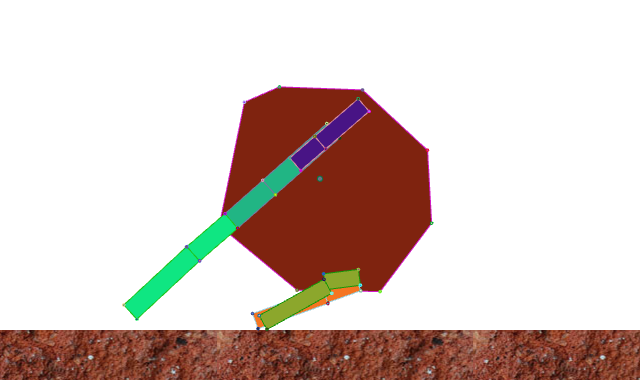
\includegraphics[width=\linewidth,center]{graphics/simulation-discussion/roll_1}
          \caption{\label{fig:roll_1}}
        \end{subfigure}
        \hspace{\fill}
        \begin{subfigure}[b]{0.3\textwidth}
          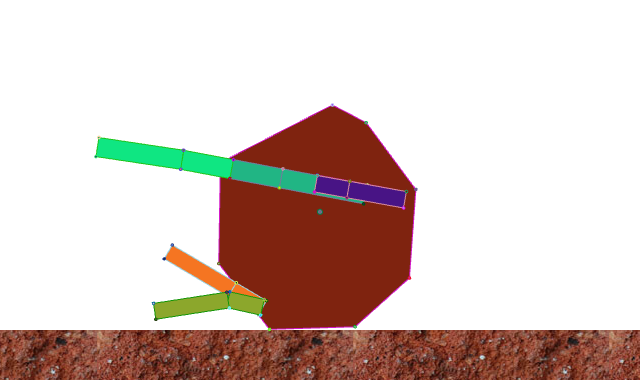
\includegraphics[width=\linewidth,center]{graphics/simulation-discussion/roll_2}
          \caption{\label{fig:roll_2}}
        \end{subfigure}
        \hspace{\fill}
        \begin{subfigure}[b]{0.3\textwidth}
          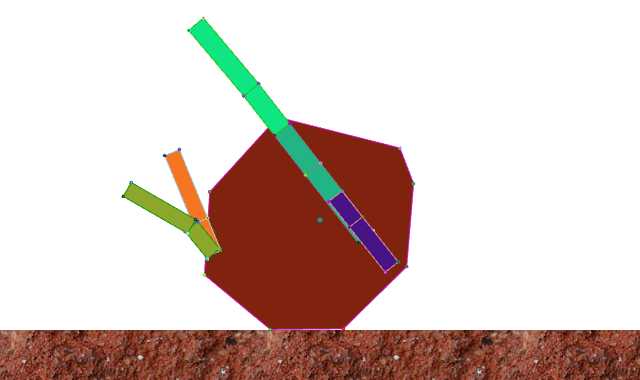
\includegraphics[width=\linewidth,center]{graphics/simulation-discussion/roll_3}
          \caption{\label{fig:roll_3}}
        \end{subfigure}

        \begin{subfigure}[b]{0.3\textwidth}
          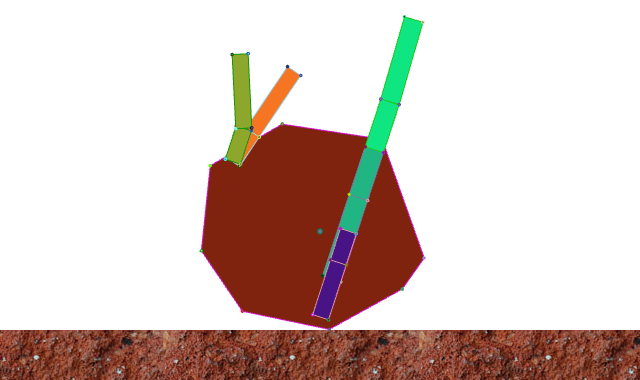
\includegraphics[width=\linewidth,center]{graphics/simulation-discussion/roll_4}
          \caption{\label{fig:roll_4}}
        \end{subfigure}
        \hspace{\fill}
        \begin{subfigure}[b]{0.3\textwidth}
          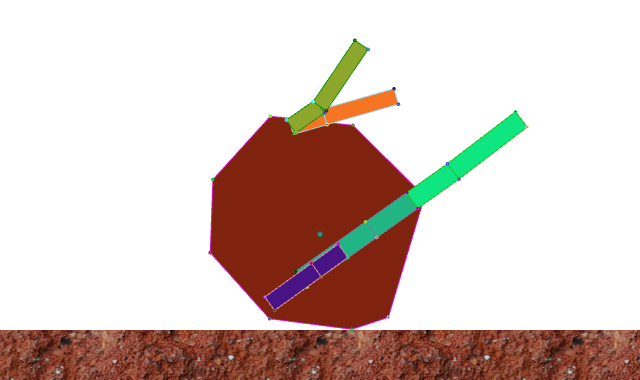
\includegraphics[width=\linewidth,center]{graphics/simulation-discussion/roll_5}
          \caption{\label{fig:roll_5}}
        \end{subfigure}
        \hspace{\fill}
        \begin{subfigure}[b]{0.3\textwidth}
          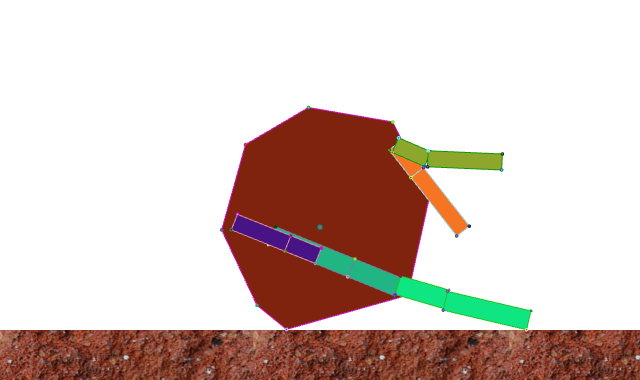
\includegraphics[width=\linewidth,center]{graphics/simulation-discussion/roll_6}
          \caption{\label{fig:roll_6}}
        \end{subfigure}

        \caption{Rollbewegung im Zeitraffer\label{fig:roll}}

      \end{figure}

      Die Hüpfbewegung in~\vref{fig:hupf} führen die Individuen aus, in dem sie sich mit einem Bein vom Boden abstossen.
      Es lässt sich keine Tendenz zu einer bestimmten Körperform erkennen.

      \begin{figure}[H]
        \centering

        \begin{subfigure}[b]{0.3\textwidth}
          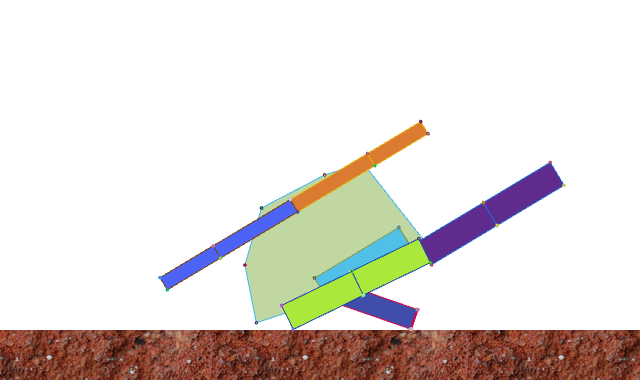
\includegraphics[width=\linewidth,center]{graphics/simulation-discussion/hupf_1}
          \caption{\label{fig:hupf_1}}
        \end{subfigure}
        \hspace{\fill}
        \begin{subfigure}[b]{0.3\textwidth}
          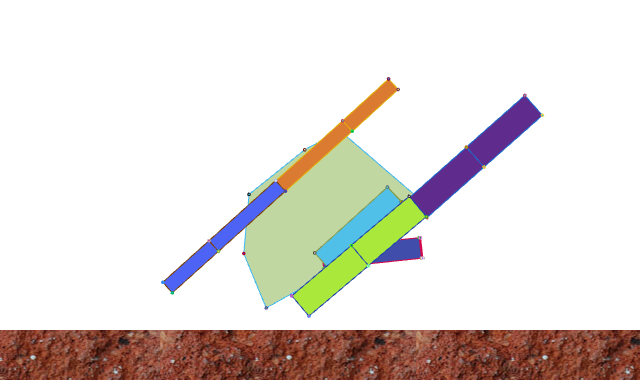
\includegraphics[width=\linewidth,center]{graphics/simulation-discussion/hupf_2}
          \caption{\label{fig:hupf_2}}
        \end{subfigure}
        \hspace{\fill}
        \begin{subfigure}[b]{0.3\textwidth}
          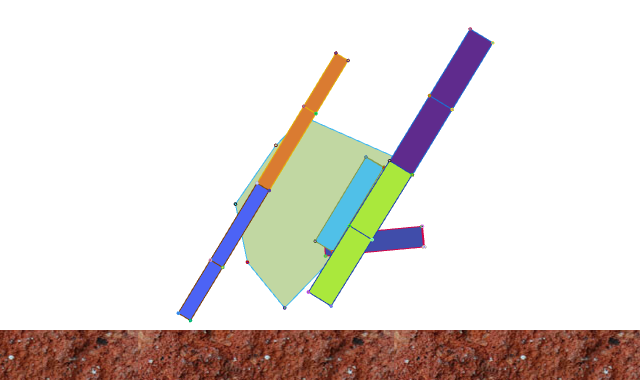
\includegraphics[width=\linewidth,center]{graphics/simulation-discussion/hupf_3}
          \caption{\label{fig:hupf_3}}
        \end{subfigure}

        \begin{subfigure}[b]{0.3\textwidth}
          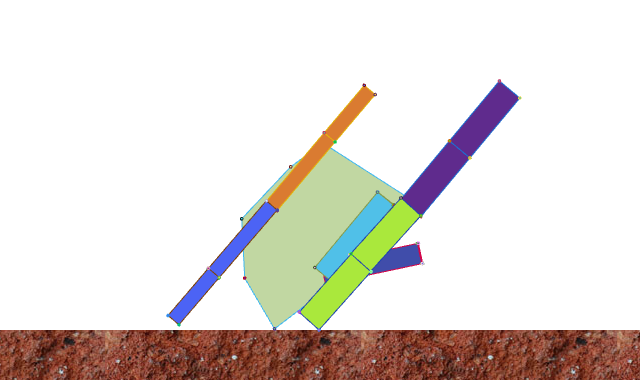
\includegraphics[width=\linewidth,center]{graphics/simulation-discussion/hupf_4}
          \caption{\label{fig:hupf_4}}
        \end{subfigure}
        \hspace{\fill}
        \begin{subfigure}[b]{0.3\textwidth}
          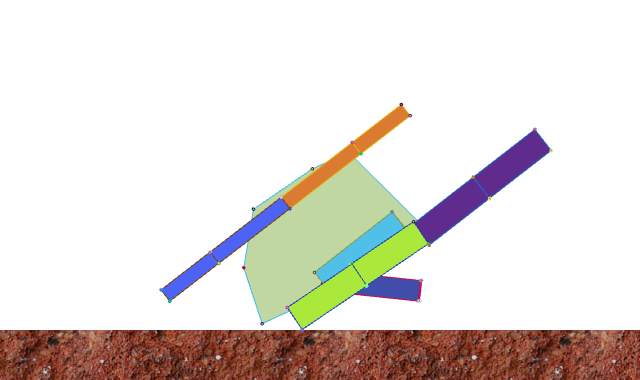
\includegraphics[width=\linewidth,center]{graphics/simulation-discussion/hupf_5}
          \caption{\label{fig:hupf_5}}
        \end{subfigure}
        \hspace{\fill}
        \begin{subfigure}[b]{0.3\textwidth}
          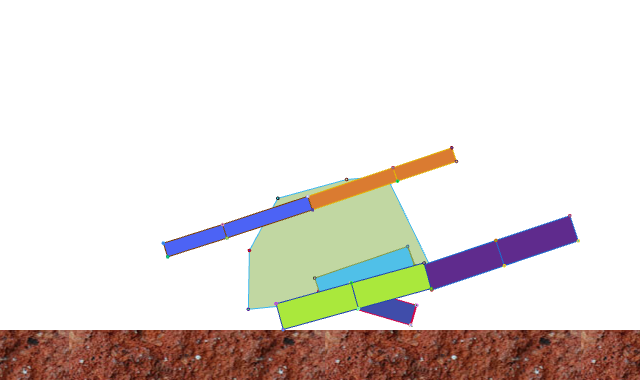
\includegraphics[width=\linewidth,center]{graphics/simulation-discussion/hupf_6}
          \caption{\label{fig:hupf_6}}
        \end{subfigure}

        \caption{Hüpfbewegung im Zeitraffer\label{fig:hupf}}

      \end{figure}

      Die Ruderer in~\vref{fig:ruder} benutzen ein Bein um die Bewegung durchzuführen,
      alle anderen Beine verharren starr am Körper.
      Die Fixierung der anderen Beine haben sie von ihren Vorfahren~(den Hüpfern) geerbt und noch nicht korrigiert.
      Es wäre von Vorteil, wenn sie alle Beine für die Ruderbewegung nutzen würden.
      Die Massen aller Beinpaare, ausser dass sich bewegende, haben sich verkleinert.
      Der Trend bei den Rundern liegt bei flachen Körpern.

      \begin{figure}[H]
        \centering

        \begin{subfigure}[b]{0.3\textwidth}
          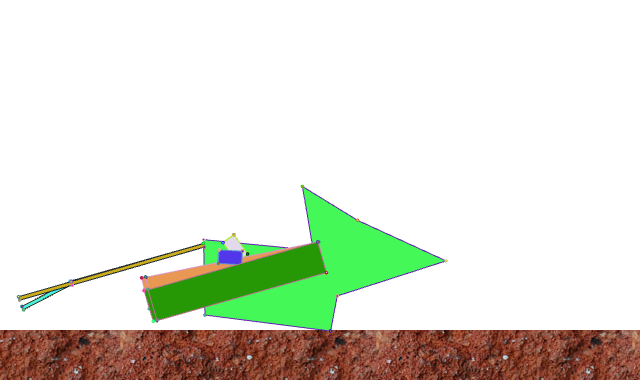
\includegraphics[width=\linewidth,center]{graphics/simulation-discussion/ruder_1}
          \caption{\label{fig:ruder_1}}
        \end{subfigure}
        \hspace{\fill}
        \begin{subfigure}[b]{0.3\textwidth}
          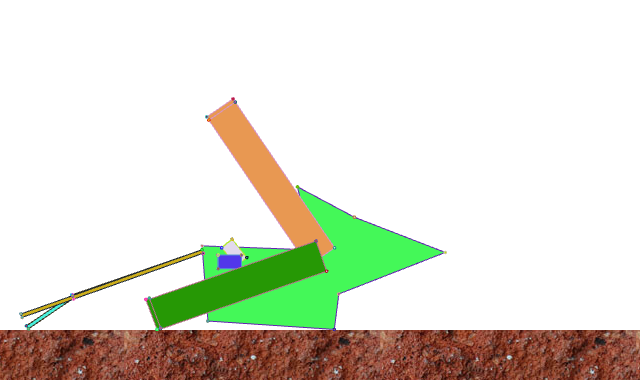
\includegraphics[width=\linewidth,center]{graphics/simulation-discussion/ruder_2}
          \caption{\label{fig:ruder_2}}
        \end{subfigure}
        \hspace{\fill}
        \begin{subfigure}[b]{0.3\textwidth}
          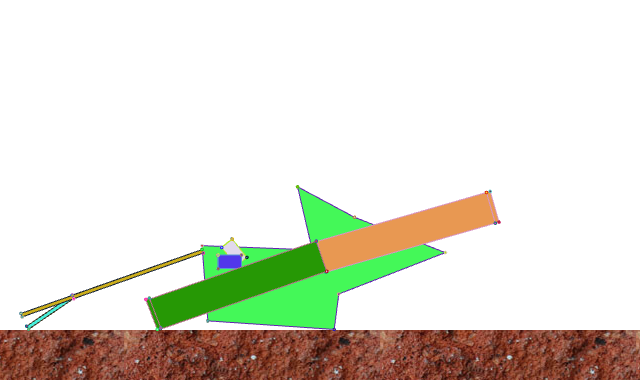
\includegraphics[width=\linewidth,center]{graphics/simulation-discussion/ruder_3}
          \caption{\label{fig:ruder_3}}
        \end{subfigure}

        \begin{subfigure}[b]{0.3\textwidth}
          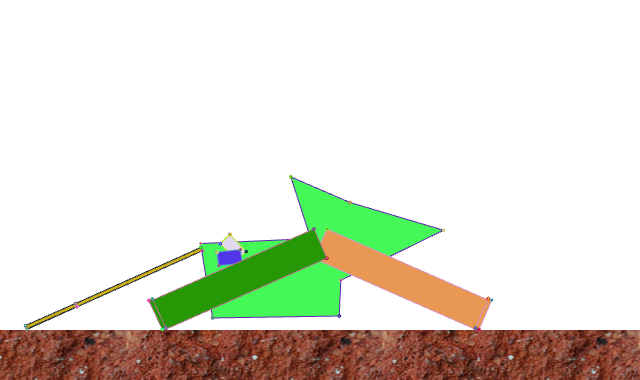
\includegraphics[width=\linewidth,center]{graphics/simulation-discussion/ruder_4}
          \caption{\label{fig:ruder_4}}
        \end{subfigure}
        \hspace{\fill}
        \begin{subfigure}[b]{0.3\textwidth}
          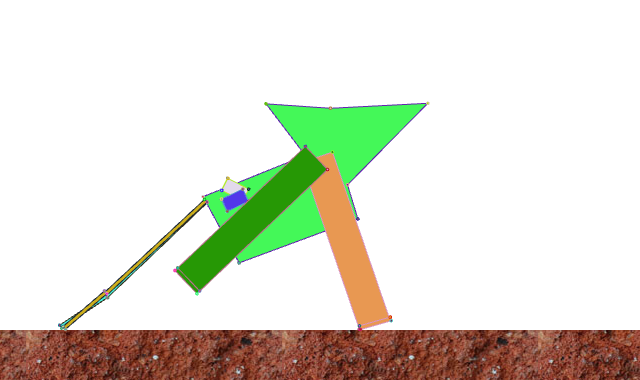
\includegraphics[width=\linewidth,center]{graphics/simulation-discussion/ruder_5}
          \caption{\label{fig:ruder_5}}
        \end{subfigure}
        \hspace{\fill}
        \begin{subfigure}[b]{0.3\textwidth}
          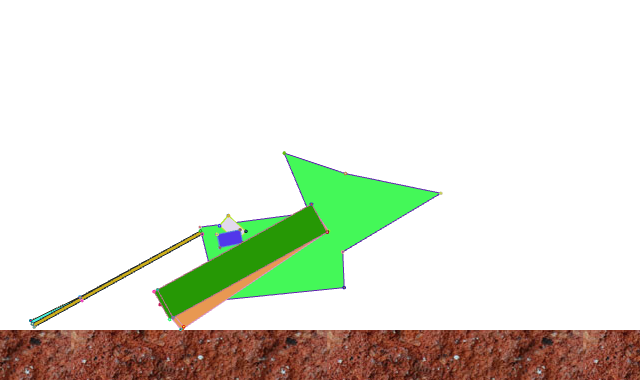
\includegraphics[width=\linewidth,center]{graphics/simulation-discussion/ruder_6}
          \caption{\label{fig:ruder_6}}
        \end{subfigure}

        \caption{Ruderbewegung im Zeitraffer\label{fig:ruder}}

      \end{figure}

      Die gefunden Resultate zeigen,
      dass nicht alle Beine benützen werden müssen, um sich durch den Parcours fortbewegen zu können.
      Eine Anpassung der Wahrscheinlichkeit für das Hinzufügen von Bewegungen (\vref{sub:wieStEv}),
      könnte die Ruderer veranlassen, alle Beine zu bewegen.
      Weiterführende Simulationen mit angepassten Parameter könnten fähig sein,
      alle Beine der artifiziellen Tiere auszunutzen.

    \subsection{Individuum: Allgemeine Lösung vs.\ Evolvieren auf Evolvierbarkeit}

      Es wird das beste Indivdiuum der 4000. Generation~(\vref{fig:gen4000}) aus dem vierten Simulationslauf~\vref{sec:4lauf}
      und dem füften Simulationslauf~(\vref{sec:5lauf}) miteinander verglichen.
      Die Individuen haben beide eine Hüpfbewegung entwickelt.
      Jedoch streckt das eine Individum~(\vref{fig:gen4000_alg}) alle Beine,
      während das Andere~(\vref{fig:gen4000_ev}) fast alle Beine angewinkelt hat.
      Das Strecken der Beine bringt eine bessere Balance,
      dies ist der Grund, warum das Individum aus der allgemeinen Lösung einen besseren Fitnesswert aufweisen kann.
      Ebenso weisst der Körper des Individuums, welches auf Evolvierbarkeit evolviert wurde, eine grössere Masse auf.
      Die Masse aller Beine ist folglich grösser beim Individum der allgemeinen Lösung.
      Während bei der Geometrie leichte Unterschiede festgestellt worden sind,
      ist die Steuerung beider Individuen fast identisch.
      \\
      Die Resulatate sprechen dafür, dass mit der allgemeinen Lösung fittere Individuen gefunden werden können.
      Um diese Aussage zu unterstreichen,
      sollten noch mehr Simulationen mit dem Evolvieren auf Evolvierbarkeit durchgeführt werden.

      \begin{figure}[H]
        \centering
        \begin{subfigure}[b]{0.45\textwidth}
          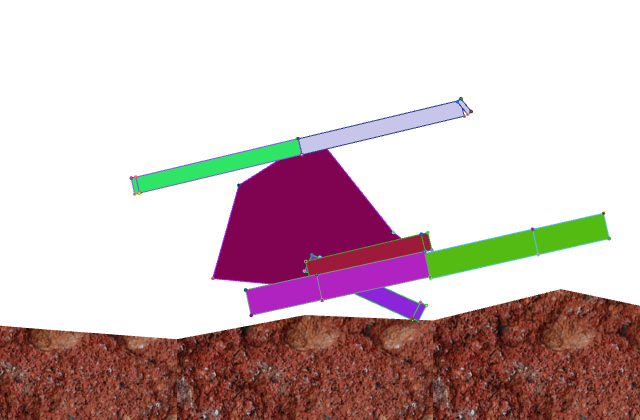
\includegraphics[width=\linewidth,center]{graphics/simulation-discussion/4_gen4000}
          \caption{Allgemeine Lösung\label{fig:gen4000_alg}}
        \end{subfigure}
        \begin{subfigure}[b]{0.45\textwidth}
          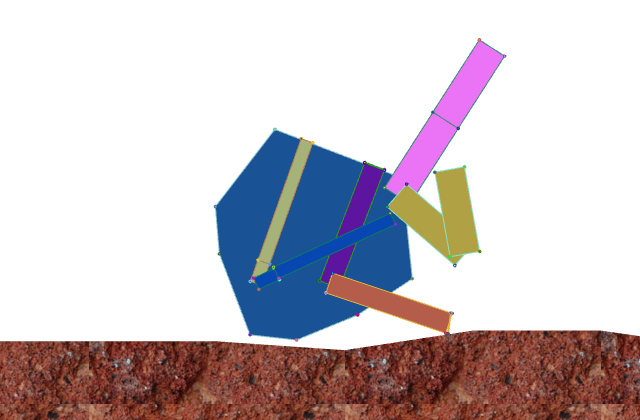
\includegraphics[width=\linewidth,center]{graphics/simulation-discussion/5_gen4000}
          \caption{Entwicklung auf Evolvierbarkeit\label{fig:gen4000_ev}}
        \end{subfigure}

        \caption{4000. Generation\label{fig:gen4000}}
      \end{figure}


    \subsection{Hypothese Körperpunkte\label{sub:PerspectiveHypBodyPoints}}

      Um eine Aussage über die Hypothese der Körperpunkte~(\vref{subsub:hypoKp}) zu treffen,
      müsste wie erwähnt unter~\vref{subsub:bpScnd} die Mutation der Anzahl Körperpunkte implementiert werden.
      Spätestens ab der 10. Generation bei jedem Simulationslauf,
      existieren nur noch Individuen mit der gleichen Anzahl Körperpunkten.
      Die Hypothese kann erst valdiert werden, wenn die Anzahl der Körperpunkte mutiert wird.

    \subsection{Hypothese Mutationswahrscheinlichkeiten}

      Die Hypothese über die Mutationswahrscheinlichkeiten~(\vref{subsub:hypoMut}) hat sich bewahrheitet
      wie in~\vref{subsub:3000gen} festgestellt worden ist.
      Kleinere Mutationswahrscheinlichkeiten tragen dazu bei, fittere Individuen zu finden.
      Hohe Mutatinswahrscheinlichkeiten bedeuten,
      dass viele Bereiche eines Individuums in einem Schritt variiert werden können.
      Dies führt dazu, dass vorteilhafte, sinnvolle Mutationen durch unvorteilhafte überschattet werden.
      Damit werden wertvolle Lösungen verspielt.

      \smallskip

      Insbesondere für die Entwicklung des Bewegungsablaufs ist dies relevant.
      Mit kleineren Wahrscheinlichkeiten werden feinere Änderungen vorgenommen,
      die in der Simulation ausgewertet werden.
      Fallen die Änderungen zu gross aus ist es möglich, dass im Ablauf eine nachteilhafte Mutation
      zu Beginn des Bewegungsablaufs eine vorteilhafte Änderung zunichtemacht.

      \smallskip

      Die Wahrscheinlichkeit der Mutation steuert,
      ob der evolutionäre Algorithmus in eine Zufallssuche abgleitet~\cite{Sampson1976}.
      Daraus folgt, dass die Wahrscheinlichkeit der entscheidende Faktor it für einen positiven oder
      negativen Effekt der Mutation.

  \section{Ausblick\label{sec:ausblick}}

    Die erstellte Simulationsapplikation ist gut erweiterbar und ermöglicht Interessierten sie weiter auszubauen.
    Der Programmcode soll für Interessierte unter \url{http://github.com} freigegeben werden.

    \subsection{Feedback an den Bewegungsmotor\label{sub:PerspectiveFeedback}}

      Eine wichtige Komponente im Bewegungsablauf stellt das Feedback dar.
      Mit einem Feedback-System können Ereignisse~(Boden berühren, Steigung und Gefällr) erkannt und verarbeitet werden.

      \smallskip

      Eine Möglichkeit ist es den Bewegungsablauf bzw.\ die Bewegung zu erweitern.
      So dass nicht nur die Bewegung weiterentwickelt wird, sondern auch wie die Rückmeldung an den Motor aussieht.
      Die Rückmeldung kann als zusätzliches Attribut einer Bewegung definiert werden.
      Das hat zur Folge, dass der Motor weiterhin als \acrshort{fsm} implementiert werden kann.
      Eine Rückmeldung ist dann eine weitere Möglichkeit für einen Zustandswechsel.
      Wobei der nächste Zustand bzw. Bewegung nicht die im Bewegungsablauf nachfolgende sein muss.
      \\
      Als weitere Option kann der Motor selbst ergänzt werden.
      Dabei steigt die Komplexität der Impelementations des Motor,
      da dieser ein Regelwerk (oder ähnlich) verwenden muss, um die Zustandswechsel zu organisieren.

      \smallskip

      In der Simulation ist bereits vorhanden, dass erkannt wird, wann ein Bein den Boden berührt.
      Diese Rückmeldung wird jedoch nicht verarbeitet.
      Es wird vermutet,
      dass die Erweiterung um ein solches System die Fitnesswerte im Verlauf der Generationen steigert.

    \subsection{\(n\)-beinige Tiere}

      % Tiere mit andere anzahl an beinen als 6

      Momentan beschränkt der definierte Bewegugngsablauf die Individuen auf sechs Beine.
      Wenn auf jedem Bein ein Bewegungsablauf definiert wird,
      wäre es möglich artifizielle Tiere mit \(n\)-Beinen zu erstellen.
      Es muss aber mit erhöhtem Rechenaufwand gerechnet werden,
      da die Bewegugnsabläufe miteinander synchronisiert werden müssen und mehr Beine bewegt werden.
      Eine weitere spannende Forschungsfrage könnte formuliert werden:
      Mit wie vielen Beine kann sich ein künstliches Tier optimal fortbewegen?

    \subsection{Austauschen der Physik-Engine}

      Eine Verbesserungsmöglichkeit ist die langsame und teilweise fehlerhafte \gls{PhysicsEngine} p2.js auszutauschen.
      Mit Hilfe einer anderen \gls{PhysicsEngine} kann schneller simuliert werden und
      es können bessere Resultate gefunden werden.
      Für einen 30 Sekunden langen Simulationslauf, benötigt die Engine zum Teil mehr als eine Minute.

    \subsection{Hypothese Selektionsstrategie\label{sub:hypoSelect}}

      Die zeitliche Beschränkung dieser Arbeit hat es nicht erlaubt,
      die ursprünglich geplante Hypothese über den Vergleich von Selektionsstrategien durchzuführen.
      In der Hypothese geht es darum die Auswirkungen von den Selektionsstrategien
      Turnierselektion, Rangselektion
      und proportionale Selektion auf die Simulationsresultate zu untersuchen.
      Diese Hypothese würde genügend Stoff für eine weitere spannende Arbeit liefern.

    \subsection{Hypothese Allgemeine Lösung vs.\ evolvieren auf Evolvierbarkeit\label{sub:hypoAnsatz}}

      Leider war nicht genügend Zeit vorhanden folgende Hypothese zu validieren:
      Individuen welche durch die allgemeine Lösung gefunden werden,
      sollten bei unterschiedlichen Parcours im Durchschnitt besser abschneiden,
      als ihre Gegenspieler~(Entwicklung auf Evolvierbarkeit),
      da sie sich schneller an eine neue Umgebung anpassen können.
      Wenn immer der gleiche Parcours benutzt wird,
      sollten die Individuen welche auf Evolvierbarkeit evolviert worden sind, auf Dauer überlegen sein.
      \\
      Um diese Hypothese zu validieren,
      sollte für beide Lösungsansätze je zwei Simulationsläufe mit 1000 Iterationen durchgeführt werden:

      \begin{itemize}
        \item Simulationslauf mit gleichem Parcours
        \item Simulationslauf mit 10 unterschiedlichen Parcours
      \end{itemize}

      Folgende Kritierien müssen erfüllt sein:

      \begin{itemize}
        \item Es sollen zwei bestehende Populationen verwendet werden.
        \item Die Parcours sollten identisch für beide Lösungsansätze sein
      \end{itemize}

      Abschliessend sollte ein Vergleich angestellt werden zwischen den Lösungsansätzen und ihrer Resultate.
      Die dafür nötige Implementierung der Parcours-Wiederverwendung ist noch offen.

    \subsection{Parcours}

      Der Parcours wird nur mit einem Typ von Element generiert, ein Höhenfeld dass einen Berg repräsentiert.
      Neue Terrain-Typen wie Eis, Wasser oder Grass könnten zusätzlich hinzugefügt werden.
      Das Hinzufügen dieser Terrain-Typen würde die Entwicklung von Individuen zulassen,
      welche sich in einer Welt bewegen, die näher an der Realität ist.
      Vergleiche könnten gezogen werden, zwischen Individuen die in verschiedenen Terrains evolviert werden.

      % ^ old, v new

      Ein Schritt in Richtung Annäherung an die Realität ist die Integration
      verschiedener Terrain-Typen in den Parcours. Der Parcours verwendet nur einen Terrain-Typ.
      Weiter Typen wie Eis, Gras, Sand oder Wasserlachen könnten hinzugefügt werden.
      \\
      Damit

      % Tendenz?

    \subsection{Neuronale Netzwerke}

      Neben den evolutinären Algorithmen gibt es noch eine andere Form von Algorithmus,
      der ähnliche Problemstellungen bewältigen kann.
      Laut M. Füllsack~\cite{book:fullsack} funktionieren neuronale Netze ähnlich wie das Neuronennetzwerk des Gehirns.
      Die bestehende Implementation des evolutionären Algorithmus könnte mit einer Version,
      welche auf neuronalen Netzwerke basiert, verglichen werden.
      Vieleicht wären neuronale Netzwerke sogar besser geeignet als die aktuelle Implementation.
      % YEEES
